% compile with XeLaTeX or LuaLaTeX
\documentclass[10pt,a5paper,twoside]{article}
\usepackage{iftex}
\RequireXeTeX
\usepackage[top=12mm,bottom=26mm,outer=28mm,inner=14mm,foot=14mm]{geometry}
\usepackage{calc}
\usepackage{scrextend}
\deffootnote[1.5em]{0em}{1em}{\thefootnotemark\quad}
\renewcommand{\footnoterule}{%
  \kern -2.4pt
  \hrule width \textwidth height 0.4pt
  \kern 2pt
}

\usepackage{fontspec}
\setmainfont[
	Ligatures=TeX,
	Extension=.otf,
	SlantedFont=cmunsl,
	BoldFont=cmunbx,
	ItalicFont=cmunti,
	BoldItalicFont=cmunbi,
	SmallCapsFont=cmunrm, % for upright instead of slanted small caps
	SmallCapsFeatures={Letters=SmallCaps,Numbers=OldStyle},	
]{cmunrm}

\usepackage{etoolbox}
\usepackage{microtype,ellipsis}

\usepackage{polyglossia,iflang}
\setotherlanguage{russian} % the name of the original Russian version at the end of this book is written using Cyrillic letters

\usepackage{textcomp}

\usepackage{amsmath,amssymb,nicefrac,amscd}
\usepackage{graphicx,float}
\usepackage{import}
\usepackage{pdfpages}

\usepackage{enumitem}
\setitemize[1]{noitemsep,nosep,leftmargin=0.99em,label={--}}

\usepackage{transparent}
\usepackage{csquotes}
\DeclareQuoteStyle{vietnamese}
  {\textquotedblleft}
  {\textquotedblright}
  [0.05em]
  {\textquoteleft}
  {\textquoteright}

\usepackage{siunitx}
\sisetup{per-mode=fraction,fraction-function=\nicefrac}

\usepackage{hyperref}

\usepackage{todonotes}

\newcommand{\eps}{\varepsilon}

% Usually, you would define a theorem-like enviroment which uses automatic numbering
% but Arnold also uses special numbering for some problems. Therefore, I kept the manual numbering.
\newenvironment{problem}[1]{\paragraph*{#1}}{}

\newenvironment{note}[1]{\par\noindent\IfLanguageName{vietnamese}{\textit{#1}}{\textsc{\MakeLowercase{#1}}} }{\par}

\makeatletter

% do no indent the first paragraph of the abstract
\let\oldabstract\abstract
\def\abstract{\oldabstract\noindent\@ifnextchar\par{\expandafter\abstract\@gobble}{}}

% always center contents of floats
\g@addto@macro\@floatboxreset{\centering}

% make all figures use 'H' position by default:
\def\fps@figure{H}
\makeatother

\usepackage{soul}
\setdefaultlanguage{dutch}
\DeclareSIUnit[number-unit-product=\,]\uur{uur}
\renewcommand{\leq}{\leqslant}
\renewcommand{\geq}{\geqslant}

\title{Oplossingen bij\\V.\,I.~Arnold's\\Opgaven voor kinderen van 5 tot 15}
\author{Rik Biel
\vspace*{1.5cm}\\
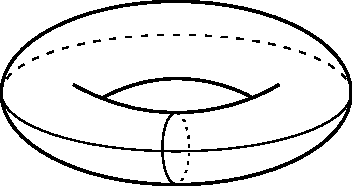
\includegraphics[scale=0.43]{resources/74_torus}
\vspace*{0.5cm}\\
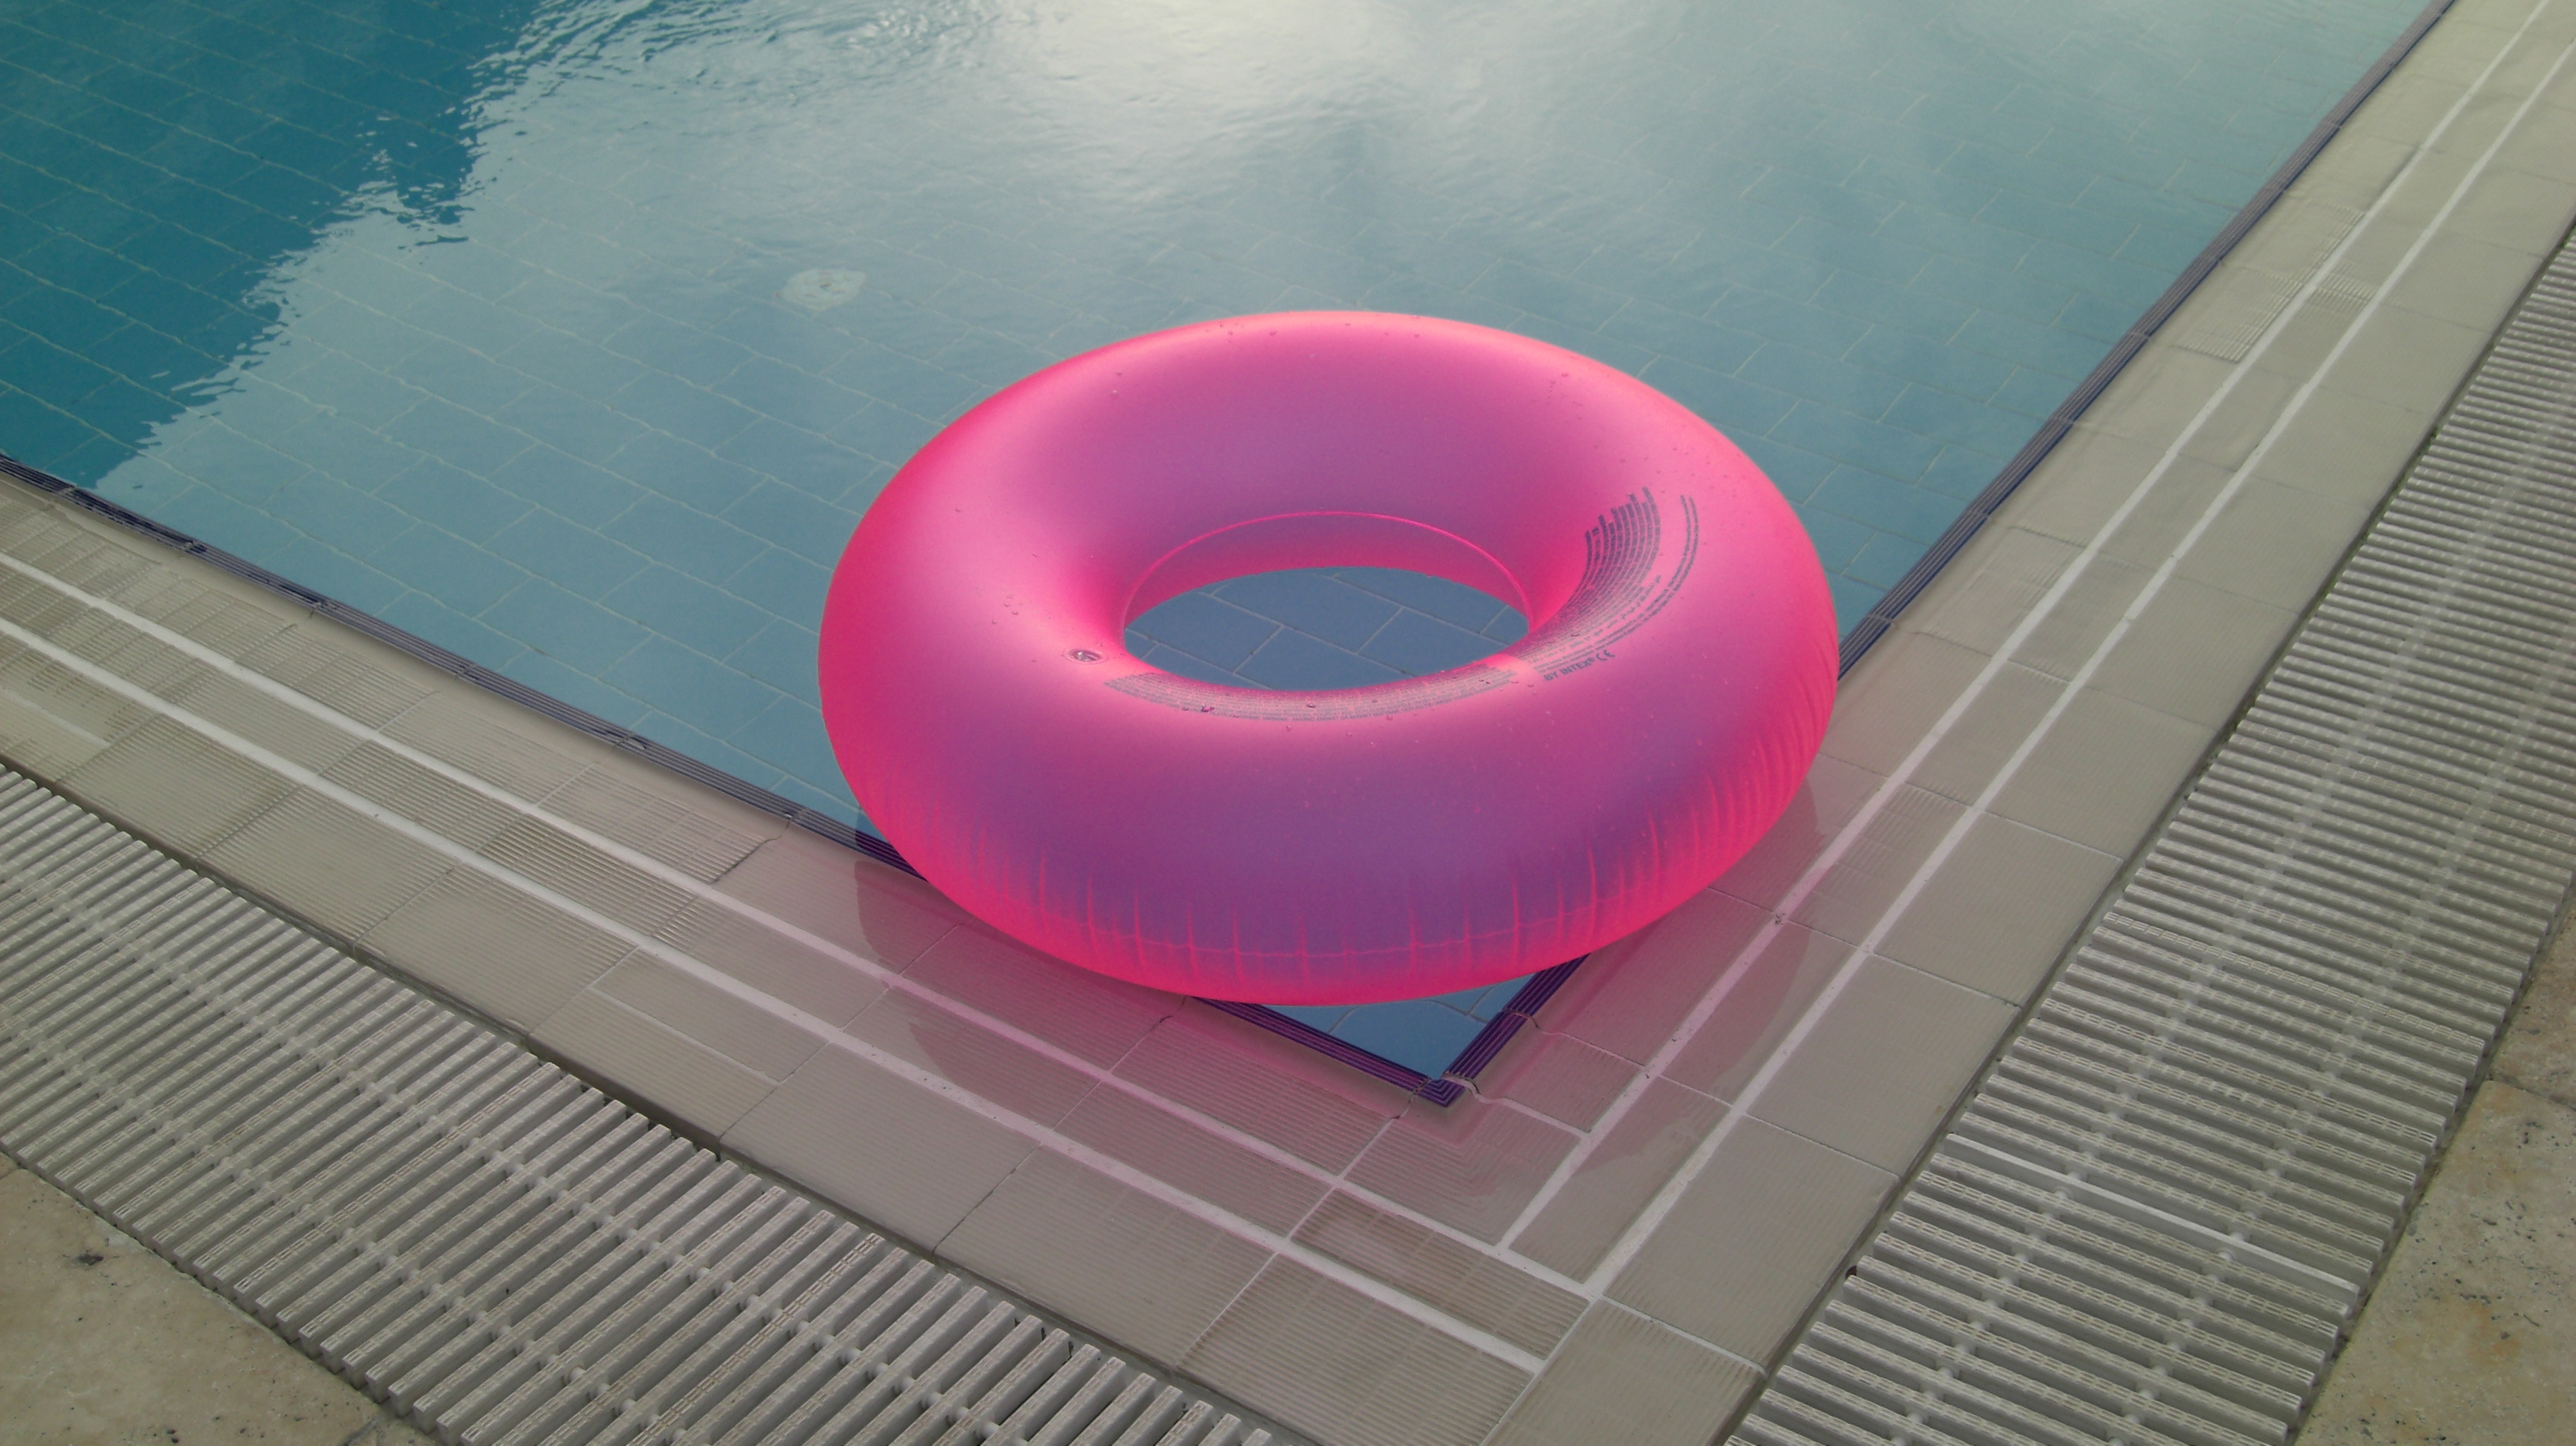
\includegraphics[scale=0.05]{resources/zwemband}
}
\date{}

\begin{document}

\maketitle
\thispagestyle{empty}
\cleardoublepage
\setcounter{page}{1}

\begin{abstract}
Dit document geeft oplossingen bij V.\,I.~Arnold's opgavenboek \href{https://www.imaginary.org/sites/default/files/5to15_nl_nl_0.pdf}{\textit{Opgaven voor kinderen van 5 tot 15}}.\\

\noindent We hebben telkens gezocht naar eenvoudige, elegante bewijzen en hebben deze in een gebalde stijl opgeschreven.
\end{abstract}

\cleardoublepage

\section*{Opmerkingen bij de oplossingen}
Sommige bewijzen lijken buiten bereik van de doelgroep van kinderen van 5 tot 15 te liggen, met name bij de \textit{formule van Cayley} (oplos\-sing~46), het \textit{Bazel-probleem} (opgave~51) en de \textit{Equidistributiestelling van Weyl} (gebruikt in oplossing~71). In die gevallen verwijzen we naar de literatuur.\\

\noindent In de volgende twee vermeldenswaardige boeken zijn van een aantal opgaven oplossingen te vinden:
\begin{itemize}
    \item V.\,I.~Arnold, \textit{Mathematical understanding of nature: essays on\\amazing physical phenomena and their understanding by\\mathematicians}, American Mathematical Society.
    \item M.~Aigner, G.\,M.~Ziegler, \textit{Proofs from THE BOOK}, Springer.
\end{itemize}

\cleardoublepage

\section*{Oplossingen}

\begin{problem}{1.}
    De kopeke die Misha tekort kwam, kon Masha blijkbaar niet bijleggen. Masha had dus geen enkele kopeke! Gegeven is dat zij er zeven tekort kwam. Het boek kostte dus zeven kopeken.
\end{problem}

\begin{problem}{2.}
    Van de 10 kopeken die de fles en de kurk samen kosten, vormen 9 het prijsverschil tussen kurk en fles. De resterende kopeke valt uiteen in twee helften: de prijs van de kurk en een deel van de prijs van de fles. De fles alleen kost dus $9 \nicefrac{1}{2}$ kopeken.
\end{problem}

\begin{problem}{3.}
    Er staat in feite dat een halve baksteen een pond weegt. De hele steen weegt dus twee pond.
\end{problem}

\begin{problem}{4.}
    Na het over en weer overgieten zijn de vloeistoffen in vat en glas mengsels geworden, maar vat en glas zijn elk wel weer precies zo vol als aan het begin. Dus bevatten ze gelijke volumes vreemde vloeistof.
\end{problem}

\begin{problem}{5.}
    Laat $t$ de tijdsduur tussen zonsopkomst en het middaguur (\SI{12}{\uur}) aangeven. De afstand die de eerste dame in $t$ uur aflegde, legde de tweede dame in $21 - 12 = 9$ uur af, dus de eerste dame was $\frac{9}{t}$ keer zo snel als de tweede dame. De afstand die de tweede dame in $t$ uur aflegde, legde de eerste in $16 - 12 = 4$ uur af, dus de eerste was $\frac{t}{4}$ keer zo snel als de tweede. De twee breuken staan voor dezelfde snelheidsverhouding: $\frac{9}{t} = \frac{t}{4}$, dus $t = 6$. De zonsopkomst was dus om $12 - t = 12 - 6 = \SI{6}{\uur}$.
\end{problem}

\begin{problem}{6.}
    De Amerikaanse scholieren gebruikten zonder verder na te denken de formule ``de oppervlakte van een driehoek is gelijk aan de basis maal de halve hoogte": $10 \cdot \frac{1}{2} \cdot 6 = 30$.

    De Russische kinderen daarentegen begrepen dat de driehoek uit de opgave helemaal niet kan bestaan. Van welke rechthoekige driehoek dan ook die op zijn schuine zijde met lengte 10 als basis ligt, is de hoogte $h$ hoogstens 5 en nooit 6. De loodlijn uit de top verdeelt de driehoek in twee rechthoekige driehoeken met rechthoekszijden $h$ en $l$, respectievelijk $h$ en $10 - l$. Driemaal de stelling van Pythagoras toepassen levert $h = \sqrt{l \cdot (10 - l)}$, met maximum $h = 5$ voor $l = 5$ (de top ligt op de halve cirkel met de basis als diameter).
\end{problem}

\clearpage

\begin{problem}{7.}
    Vasya niet meegerekend, is het aantal meisjes in het gezin 2 groter dan het aantal (nul of meer) jongens. Vasya is zelf een jongen, dus in het hele gezin is er 1 meisje meer dan dat er jongens zijn.
\end{problem}

\begin{problem}{8.}
    De oppervlakte van de bloem verdubbelt zich elke dag. Op 1~juli is de hele vijver bedekt, dus de helft was bedekt op de dag ervoor, op 30~juni.
\end{problem}

\begin{problem}{9.}
    De boer zet eerst de geit over, vaart terug, zet vervolgens de wolf over, neemt de geit mee terug, brengt de kool over, vaart weer terug, en neemt ten slotte de geit nog een keer mee naar de overkant.
\end{problem}

\begin{problem}{10.}
    De slak stijgt $3 - 2 = \SI{1}{\cm}$ per etmaal. Aan het begin van dag~998 zit hij op een hoogte van \SI{9}{\metre} en \SI{97}{\cm}. Gedurende die dag klimt hij \SI{3}{\cm} tot \SI{10}{\metre} hoogte en bereikt hij de top van de paal met het hapje.
\end{problem}

\begin{problem}{11.}
    De voor de hand liggende oplossing voor de plek van de tent is de noordpool. De beer was dus een ijsbeer, dus wit.

    Daarnaast zijn er oneindig veel oplossingen in de buurt van de zuidpool. Beschouw daar breedtecirkels $C_n$ met omtrek \SI{10}{\km}$/n$, voor $n = 1,2,\dotsc$. Als de tent zich bevindt op een willekeurig punt op de breedtecirkel \SI{10}{\km} ten noorden van zo'n cirkel $C_n$ (gemeten over het aardoppervlak), dan kan de opgegeven weg worden afgelegd. De \SI{10}{\km} oostwaarts bestaat uit het $n$ keer doorlopen van $C_n$.
\end{problem}

\begin{problem}{12.}
    Het tij wordt vooral bepaald door de zwaartekracht van de maan. De maan draait in ongeveer 30 dagen om de aarde, met de draaiing van de aarde mee. Omdat de maan vooruitloopt op de aarde, heeft een bepaalde plaats op aarde de volgende dag pas ongeveer $\nicefrac{1}{30}$ dag oftewel 48 minuten later weer dezelfde positie ten opzichte van de maan. Het antwoord is dus rond \SI{12.48}{\uur}.
\end{problem}

\begin{problem}{13.}
    We nemen aan dat de twee boeken op volgorde staan, dus dat het tweede deel rechts van het eerste deel staat. Bekijk of teken deze situatie! Je ziet dat er zich tussen de eerste bladzijde van het eerste deel en de laatste bladzijde van het tweede deel alleen de voorkaft van het eerste deel en de achterkaft van het tweede deel bevinden. De twee kaften zijn samen \SI{4}{\mm} dik.
\end{problem}

\clearpage

\begin{problem}{14.}
    Er zijn vele oplossingen. De figuur toont een mogelijk zijaanzicht van een lichaam dat het gevraagde voor- en bovenaanzicht heeft.\\

    \hspace{3cm}
    \begin{tikzpicture}[thick,scale=0.8]
        \draw (0,0) -- (3,0) -- (3,3) -- (2,2.5) -- (1,3) -- (0,3) -- (0,0);
        \draw (0,3) -- (0.5,0);
        \draw (0,3) -- (1,0);
    \end{tikzpicture}
\end{problem}

\begin{problem}{15.}
    ???
\end{problem}

\begin{problem}{16.}
    We beschouwen een trap van $n+1$, $n \geq 1$, gestapelde staven van lengte 1, genummerd van boven naar beneden: $k = 1$ is de hoogste staaf en $k = n+1$ de laagste. Elke staaf $k$, $1 \leq k \leq n$, heeft een overhang $x_k \geq 0$ ten opzichte van de onderliggende staaf $k+1$.

    Met $z_k$, $1 \leq k \leq n$, geven we de horizontale afstand aan tussen het zwaartepunt van de bovenste $k$ staven en het midden van staaf $k+1$: $z_1 = x_1$ en $z_k = (x_k + (k - 1) (x_k + z_{k-1})) / k = x_k + \left( \frac{k-1}{k} \right) z_{k-1}$ voor $1 < k \leq n$.

    De voorwaarde voor stabiliteit van de hele stapel is $z_k \leq \frac{1}{2}$ voor alle $1 \leq k \leq n$. We zoeken de grens op: $z_k = \frac{1}{2}$ voor alle $1 \leq k \leq n$. Dan volgt $x_k = \frac{1}{2} \left( 1 - \frac{k-1}{k} \right) = \frac{1}{2 k}$, $1 \leq k \leq n$. De totale overhang is:
    \begin{equation*}
        x = \textstyle\sum\limits_{k=1}^{n} x_k = \frac{1}{2} \textstyle\sum\limits_{k=1}^{n} \frac{1}{k}.
    \end{equation*}
    Het is bekend dat de harmonische reeks $\sum\limits_{k=1}^{\infty} \frac{1}{k}$ divergeert, dus $x$ kan willekeurig groot zijn door $n$ groot genoeg te nemen en $x_k = \frac{1}{2 k}$.
\end{problem}

\begin{problem}{17.}
    De onderlinge afstand van de twee fietsers is aanvankelijk \SI{40}{\km} en neemt af met $10 + 15 = \SI{25}{\km\per\uur}$. Ze treffen elkaar dus na $\nicefrac{40}{25} = 1{,}6 \text{ uur}$. In die tijd legt de vlieg $100 \cdot 1{,}6 = \SI{160}{\km}$ af.
\end{problem}

\begin{problem}{18.}
    Dat is niet mogelijk. Neem 31 dominostenen met een witte en een zwarte helft. Deze kunnen op een schaakbord altijd kleur op kleur worden gelegd (waar dat niet het geval is, is dat op te lossen door een steen andersom te leggen), en laten één wit veld en één zwart veld onbedekt. Tegenoverliggende hoekvelden op dezelfde diagonaal hebben echter dezelfde kleur.
\end{problem}

\clearpage

\begin{problem}{19.}
    De rups moet hoe dan ook over twee zijvlakken van de kubus kruipen. Dat kan via zes combinaties van twee zijvlakken. Worden de twee vlakken in gedachten plat neergelegd als een rechthoek, dan komen begin- en eindpunt van de weg overeen met schuin tegenover elkaar liggende hoekpunten. De kortste weg daartussen -- een rechte lijn -- is een diagonaal van de rechthoek (met lengte $\sqrt{5}$ maal de lengte van de ribbe van de kubus). De overeenkomende weg op de kubus kruist een ribbe in het midden.
\end{problem}

\begin{problem}{20.}
    Vul het 3 liter vat volledig met water en giet het leeg in het 5~liter vat. Vul het 3 liter vat nogmaals volledig en giet daaruit zoveel in het 5 liter vat tot dat vol is. Het restant in het 3 liter vat is één liter.
\end{problem}

\begin{problem}{21.}
    Bij elk hoofd hoort minstens één paar benen, dus bij vijf hoofden horen minstens tien benen. Dan zijn er nog twee paar benen over, dus er zijn twee honden. De overige hoofden en benen zijn goed voor drie mensen.
\end{problem}

\begin{problem}{22.}
    Deze uitspraak staat bekend als de \textit{Stelling van Napoleon}. We geven een aanschouwelijk bewijs. We draaien één van de gelijkzijdige driehoeken om elk van de centra van de twee andere, over $\nicefrac{2 \pi}{3}$ radialen, in tegengestelde richtingen zodat de beelden samenvallen. De grijze driehoeken in de figuur zijn dan gelijkbenig, met hoeken van $\nicefrac{\pi}{6}$ en $\nicefrac{2 \pi}{3}$ radialen, en even groot. Daaruit volgt dat de driehoek die wordt bepaald door de centra $*$, hoeken van $\nicefrac{\pi}{3}$ radialen heeft en dus gelijk\-zijdig is.
    \begin{figure}
		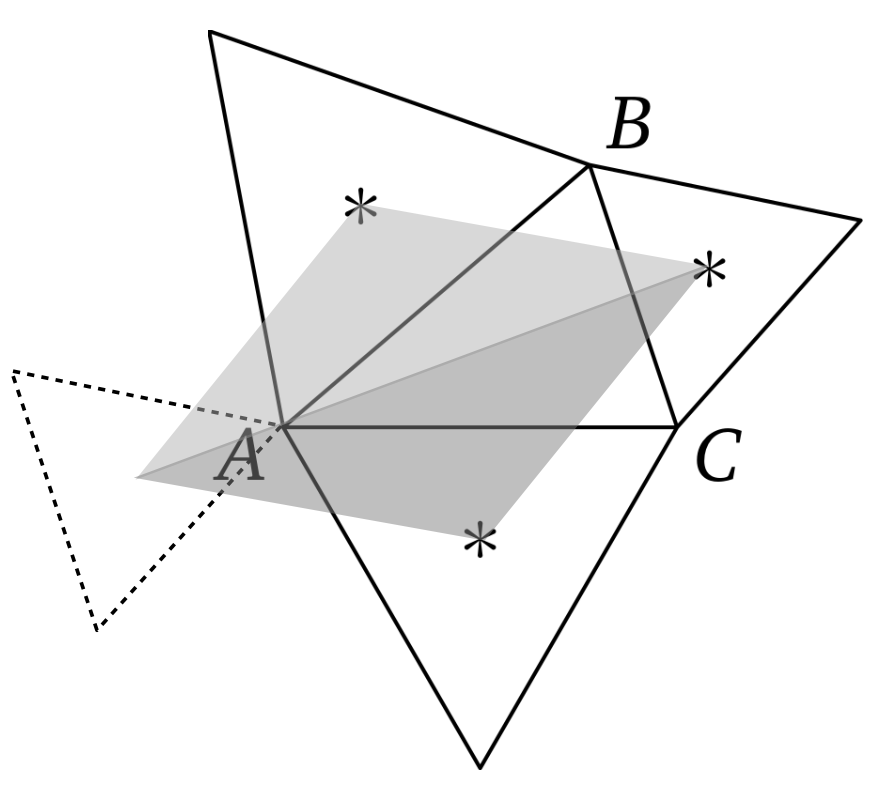
\includegraphics[scale=0.15]{resources/oplossing22}
	\end{figure}
\end{problem}

\clearpage

\begin{problem}{23.}
    Omdat een kubus zes zijvlakken heeft, zijn zevenhoeken niet mogelijk. De figuur in de opgave toont een willekeurige driehoek. Het is eenvoudig in te zien dat ook gelijkbenige en gelijkzijdige driehoeken mogelijk zijn. Vierhoeken, rechthoeken, een vierkant, vijfhoeken en zeshoeken zijn ook mogelijk. Een zeshoek is regelmatig als het platte vlak de ribben in hun midden snijdt. Een regelmatige vijfhoek is niet mogelijk.
\end{problem}

\begin{problem}{24.}
	Neem zonder verlies van algemeenheid de kubus met de oor\-sprong $(0,0,0)$ als centrum en de acht hoekpunten $(\pm l,\pm l,\pm l)$ op afstand 1 van de oorsprong, dus $l = \nicefrac{1}{\sqrt{3}}$. Beschouw lijnen door de oorsprong met hun richtingen bepaald door punten $(e_1,e_2,e_3)$ op afstand 1 van de oorsprong, dus $\sum\limits_{j=1}^{3} {e_j}^2 = 1$. Van de hoeken $\alpha_n$, $n = 1,\dotsc,8$, tussen een bepaalde lijn en de lijnstukken van de oorsprong naar de hoekpunten van de kubus zijn $\cos \alpha_n = \sum\limits_{j=1}^{3} \pm l \cdot e_j$, volgens de formule voor het inwendig product. De afstanden tussen de hoek\-punten en deze lijn bedragen $\sin \alpha_n$. De som van hun kwadraten is:\\$\sum\limits_{n=1}^{8} \sin^2 \alpha_n = \sum\limits_{n=1}^{8} (1 - \cos^2 \alpha_n) = 8 - \sum\limits_{(\pm l,\pm l,\pm l)} {\left( \sum\limits_{j=1}^{3} \pm l \cdot e_j \right)}^2\\= 8 - 8 l^2 \sum\limits_{j=1}^{3} {e_j}^2 - \sum\limits_{(\pm l,\pm l,\pm l)} \sum\limits_{j,k=1;j \neq k}^{3} \pm l \cdot e_j \cdot \pm l \cdot e_k = \nicefrac{16}{3}$\\(de 48 termen van de laatste som vallen tegen elkaar weg). Deze uitkomst is onafhankelijk van $(e_1,e_2,e_3)$, dus voor alle lijnen gelijk.
\end{problem}

\clearpage

\begin{problem}{25.}
	Het blijkt dat de snijkromme een ellips is met $A$ en $B$ als brand\-punten. Voor elk punt op een ellips is de som van diens afstanden tot de brandpunten gelijk.\\

    Vanaf een willekeurig punt buiten een bol is de afstand langs elke raaklijn aan de bol tot het raakpunt gelijk. Dit passen we toe op elk punt van de snijkromme en beide \textit{bollen van Dandelin}, met lijnstukken naar de raakpunten $A$ en $B$, en lijnstukken langs een beschrijvende lijn van de kegel naar elk van beide cirkels waar de bollen de kegel raken: in de figuur zijn de groene lijnstukken even lang en zijn de rode lijnstukken even lang.

    De som van de lengten van deze lijnstukken, het groene en het rode lijnstuk (beschouw deze op de beschrijvende lijn van de kegel), is voor alle punten op de snijkromme gelijk, omdat de genoemde cirkels gecentreerd zijn op de as van de kegel en in evenwijdige vlakken loodrecht op deze as liggen.

    Dus op de snijkromme is de som van de afstanden tot $A$ en $B$ constant, dus de kromme is een ellips met brandpunten $A$ en $B$.
    \begin{figure}
		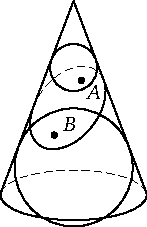
\includegraphics{resources/taskbook-9}
        \hspace{2cm}
		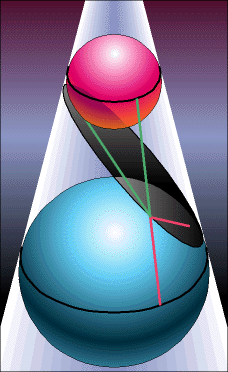
\includegraphics[scale=0.4]{resources/DandelinSpheres}

        \rightline{\scriptsize{Met dank aan: \href{https://commons.wikimedia.org/wiki/File:DandelinSpheres.png?uselang=nl}{DandelinSpheres}, via Wikimedia Commons.}}
	\end{figure}
\end{problem}

\clearpage

\begin{problem}{26.}
    Beschouw een smalle strook op het aardoppervlak rond breedte\-graad $\phi$.

    Is $R$ de straal van de aarde, dan heeft de betreffende breedtecirkel straal $R \cos \phi$. Dus de verhouding van de omtrek van de projectie van de breedtecirkel op de cilindermantel en de omtrek van de breedte\-cirkel zelf is $\nicefrac{1}{\cos \phi}$.

    De raaklijn aan elke meridiaan in het snijpunt met de betreffende breedtecirkel maakt een hoek $\phi$ met de lijn door dit punt evenwijdig aan de cilinderas. Dus de verhouding van de breedte van de projectie van het strookje op de cilindermantel en de breedte van het strookje zelf is $\cos \phi$.

    Samengevat is deze projectie een oppervlaktegetrouwe afbeelding: $\cos \phi \cdot \nicefrac{1}{\cos \phi} = 1$. In het bijzonder heeft de projectie van Frankrijk dezelfde oppervlakte als het land zelf.
\end{problem}

\begin{problem}{27.}
    Met het \textit{binomium van Newton} kunnen we schrijven:
    \begin{equation*}
        2^p = {(1+1)}^p = \textstyle\sum\limits_{k=0}^{p} \binom{p}{k}\, 1^{p-k}\, 1^k = \textstyle\sum\limits_{k=0}^{p} \frac{p!}{k!\, (p-k)!}.
    \end{equation*}
    Dit kan worden uitgewerkt tot:
    \begin{equation*}
        2^p = 2 + 2 p \textstyle\sum\limits_{k=1}^{\nicefrac{(p-1)}{2}} \frac{(p-1)!}{k!\, (p-k)!}.
    \end{equation*}
    Halveren levert de gezochte betrekking:
    \begin{equation*}
        2^{p-1} = p \left( \textstyle\sum\limits_{k=1}^{\nicefrac{(p-1)}{2}} \frac{(p-1)!}{k!\, (p-k)!} \right) + 1 = p\, a + 1, \text{ met } a \text{ geheel}.
    \end{equation*}
    In deze afleiding zijn twee punten doorslaggevend. Omdat $p$ oneven is, is $\frac{p-1}{2}$ geheel. Omdat $p$ priem is, zijn $\frac{(p-1)!}{k!\, (p-k)!}$ geheel (binomiaal\-coëfficiënten zijn geheel, in $\binom{p}{k} = \frac{p!}{k!\, (p-k)!} = \frac{p \cdot (p-1) \cdot \dots \cdot (p-k+1)}{k \cdot (k-1) \cdot \dots \cdot 1}$ is $p$ wel een priemdeler van de teller maar niet van de noemer, dus zijn $\frac{1}{p} \binom{p}{k} = \frac{(p-1)!}{k!\, (p-k)!}$ ook geheel).
\end{problem}

\clearpage

\begin{problem}{28.}
    Deze opgave staat bekend als het \textit{naaldprobleem van Buffon}.

    Laat $l$ de waarde zijn van de regelafstand en de naaldlengte; de precieze waarde, hier 10, maakt niet uit. Twee parameters bepalen de positie van de gevallen naald ten opzichte van de lijnen op het papier: de hoek $\phi$, $0 \leq \phi \leq \frac{\pi}{2}$, tussen de richting van de naald en de richting loodrecht op de lijnen, en de afstand $d$, $0 \leq d \leq \frac{l}{2}$, van het midden van de naald tot de dichtstbijzijnde lijn. De projectie van de naald loodrecht op de lijnen heeft lengte $l \cos \phi$. De naald kruist de dichtstbijzijnde lijn als $d \leq \frac{l}{2} \cos \phi$. De $(\phi,d)$ rechthoek heeft oppervlakte $\frac{\pi}{2} \cdot \frac{l}{2} = \frac{\pi l}{4}$. Het deel $d \leq \frac{l}{2} \cos \phi$ heeft oppervlakte $\frac{l}{2} \int_{0}^{\frac{\pi}{2}} \cos \phi \,d \phi = \frac{l}{2}$. De kans dat de naald een lijn kruist is gelijk aan de verhouding van de oppervlakten: $\frac{l}{2} / \frac{\pi l}{4} = \frac{2}{\pi}$.

    Laat nu de naald licht gekromd zijn met $a \cdot l$, $0 \ll a < 1$, de afstand tussen de uiteinden van de naald. De kans dat de naald een lijn kruist is nu: $\frac{a \cdot l}{2} / \frac{\pi l}{4} = \frac{2 a}{\pi}$.
\end{problem}

\begin{problem}{29.}
    Voor convexe veelvlakken met $H$ hoekpunten, $R$ ribben en $Z$~zij\-vlakken geldt de \textit{formule van Euler}: $H - R + Z = 2$.

    Wanneer alle zijvlakken driehoeken zijn, dan horen er bij elk zijvlak drie ribben en bij elke ribbe twee zijvlakken (voor de hoekpunten kunnen we niet soortgelijke uitspraken doen). Het is niet zo dat het veelvlak drie keer zoveel ribben als zijvlakken heeft of twee keer zoveel zijvlakken als ribben, omdat er in die tellingen dubbelingen zitten. De genoemde verhoudingen gelden wel voor het aantal (ongeordende) paren van zijvlak en ribbe. Dit aantal is gelijk aan $3 Z$ en ook gelijk aan $2 R$, dus $3 Z = 2 R$. In dit geval luidt de formule van Euler: $Z = 2 H - 4$.\\Zie in de figuur in de opgave de tetraëder: $H = 4,R = 6,Z = 4$, octaëder: $H = 6,R = 12,Z = 8$, icosaëder: $H = 12,R = 30,Z = 20$.
\end{problem}

\clearpage

\begin{problem}{30.}
    In de figuur is een kubus in een dodecaëder getekend. De dode\-caëder heeft 12 zijvlakken en de kubus 12 ribben. Van elk zijvlak van de dodecaëder valt één van de diagonalen samen met een ribbe van de kubus. Omdat elk zijvlak van de dodecaëder vijf diagonalen heeft, zijn er vijf van zulke kubussen te onderkennen.
    \begin{figure}
        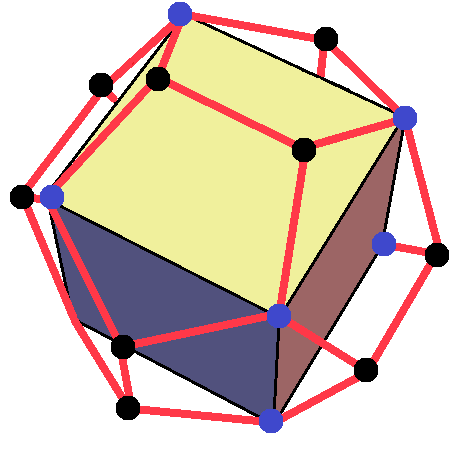
\includegraphics[scale=0.28]{resources/Cube_in_dodecahedron}

        \scriptsize{Met dank aan: \href{https://commons.wikimedia.org/wiki/File:Cube_in_dodecahedron.png?uselang=nl}{Tomruen}, \href{https://creativecommons.org/licenses/by-sa/4.0}{CC BY-SA 4.0}, via Wikimedia Commons.}
    \end{figure}
    De figuur maakt ook inzichtelijk dat een dodecaëder kan worden gevormd door op elk zijvlak van een kubus een dakje te plaatsen.
\end{problem}

\begin{problem}{31.}
    De doorsnede van de twee tetraëders is een octaëder, waarvan de hoekpunten op de middens van de zijvlakken van de kubus liggen.
    \begin{figure}
        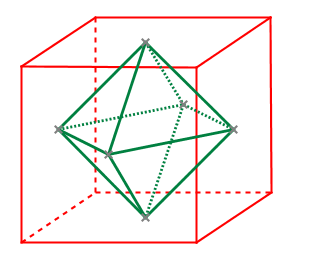
\includegraphics[scale=0.35]{resources/Octahedron_in_Cube}

        \scriptsize{Met dank aan: \href{https://commons.wikimedia.org/wiki/File:Octahedron_in_Cube.png?uselang=nl}{Birgit Lachner}, \href{http://creativecommons.org/licenses/by-sa/3.0/}{CC BY-SA 3.0}, via Wikimedia Commons.}
    \end{figure}
    Een octaëder bestaat uit twee piramides. De inhoud van een (wil\-lekeurige) piramide is gelijk aan $\frac{1}{3}$ maal de oppervlakte van het grond\-vlak maal de hoogte. Heeft de kubus inhoud 1, dan heeft elk van beide piramides inhoud $\frac{1}{3} \cdot \frac{1}{2} \cdot \frac{1}{2} = \frac{1}{12}$, dus de octaëder inhoud $\frac{1}{6}$.
\end{problem}

\clearpage

\begin{problem}{31\textsuperscript{bis}.}
	De doorsnede is een (onregelmatige) zeshoek, waarvan de drie gegeven punten hoekpunten zijn en waarvan tegenoverliggende zijden evenwijdig zijn. De figuur toont een `constructie zonder woorden' om eerst één van de drie onbekende hoekpunten te bepalen en daarna de andere twee.
    \begin{figure}
        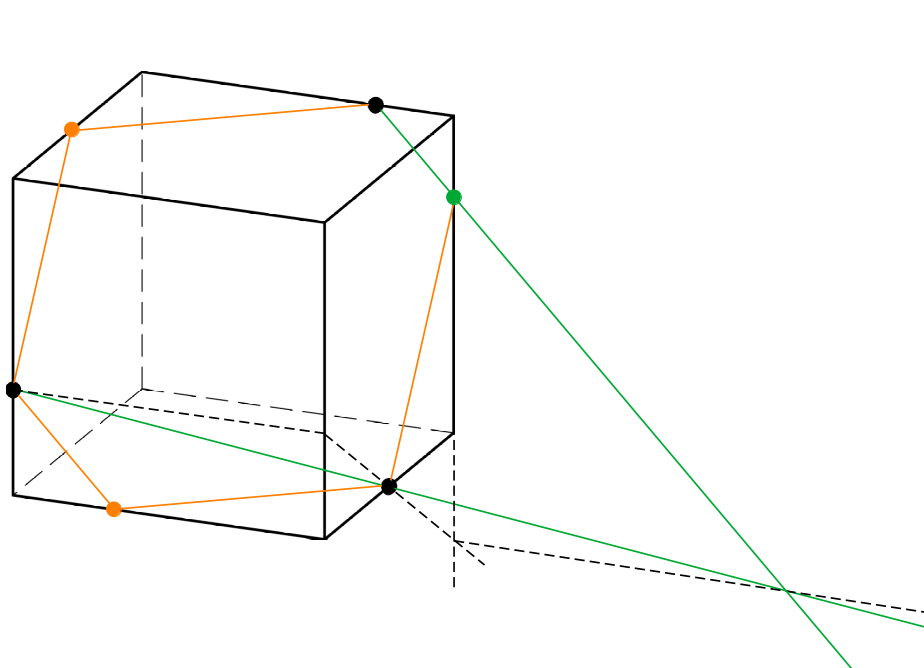
\includegraphics[scale=0.2]{resources/oplossing31bis}
    \end{figure}
\end{problem}

\begin{problem}{32.}
	Een regelmatig veelvlak heeft $Z$ zijvlakken ($Z = 4,6,8,12,20$) en per zijvlak $N$ zijden (of hoekpunten) (resp. $N = 3,4,3,5,3$). Een bepaald zijvlak kan door $Z$ draaiingen worden overgevoerd in alle zijvlakken (met inbegrip van de identiteit die het lichaam ongemoeid laat) en vervolgens gedraaid in $N$ standen, waarna het lichaam weer dezelfde ruimte inneemt als aan het begin. Dit zijn $Z N$ draaiingen. Daarbovenop kan elk van deze uitkomsten binnenstebuiten worden gekeerd. Dit zijn $Z N$ spiegelingen. Dus samen $2 Z N$ symmetrieën.

    Analoge betogen zijn er met $H$ hoekpunten ($H = 4,8,6,20,12$) en $M$ ribben (of zijvlakken) per hoekpunt (resp. $M = 3,3,4,3,5$) en dan $2 H M$ symmetrieën, of met $R$ ribben ($R = 6,12,12,30,30$) en 2~zijvlakken (of hoekpunten) per ribbe en dan $4 R$ symmetrieën.

    Dus een tetraëder heeft 24 symmetrieën, een kubus en een octaëder hebben er 48, en een icosaëder en een dodecaëder 120, waarvan telkens de helft draaiingen zijn en de helft spiegelingen.
\end{problem}

\clearpage

\begin{problem}{33.}
    Kies, zonder verlies van algemeenheid, één van de zes kleuren voor het bovenvlak van de kubus. Voor het ondervlak zijn er dan 5 mogelijke kleuren. Kies vervolgens, weer zonder verlies van algemeen\-heid, één van de overgebleven vier kleuren voor één van de vier zij\-vlakken. Voor het zijvlak ertegenover zijn er dan 3 mogelijke kleuren. Voor het verdelen van de twee overgebleven kleuren over de twee overgebleven zijvlakken zijn er 2 mogelijkheden. Het totaal aantal mogelijkheden is $5 \cdot 3 \cdot 2 = 30$.
\end{problem}

\begin{problem}{34.}
    Het aantal mogelijkheden om $n$ voorwerpen te rangschikken is $n$-faculteit:
    \begin{equation*}
        n! = n \cdot (n - 1) \cdot (n - 2) \cdot \dots \cdot 2 \cdot 1 = \textstyle\prod\limits_{k=1}^{n} k.
    \end{equation*}
    Voorbeelden: $4! = 1 \cdot 2 \cdot 3 \cdot 4 = 24$, $5! = 1 \cdot 2 \cdot 3 \cdot 4 \cdot 5 = 120$, $6! = 5! \cdot 6 = 120 \cdot 6 = 720$, $10! = \Pi_{k=1}^{10} k = 3\,628\,800$.
\end{problem}

\begin{problem}{35.}
	Elke draaiing van de kubus geeft een permutatie van zijn vier lichaamsdiagonalen. De vraag is of ze allemaal verschillend zijn. Elke permutatie kan maar op één manier in zichzelf overgaan (naast de identieke afbeelding, die alles op zijn plaats laat), namelijk door een puntspiegeling in het centrum van de kubus. De puntspiegeling is niet door draaiingen te verwezenlijken. Er zijn dus evenveel permutaties als draaiingen, en dat zijn er 24 (de identieke afbeelding meegerekend); Mark Ronan legt dit heel mooi uit in \href{http://www.markronan.com/mathematics/symmetry-corner/the-rotations-of-a-cube/}{The Rotations of a Cube}. Zie ook oplossing~32.
\end{problem}

\begin{problem}{36.}
    Het genoemde verschil is een veelvoud van 3. Voor $n$ willekeurige gehele getallen $a_1,a_2,\dotsc,a_n$ bestaat er een geheel getal $b_n$ zodat:
    \begin{equation*}
        {(a_1 + a_2 + \dots + a_n)}^3 - ({a_1}^3 + {a_2}^3 + \dots + {a_n}^3) = 3 b_n.
    \end{equation*}
    Bewijs via volledige inductie:
    \begin{itemize}
        \item Voor $n = 1$ is $b_1 = 0$.
        \item Vervolgens nemen we de stap van $n$ naar $n + 1$:\\
            ${(a_1 + \dots + a_{n+1})}^3 - ({a_1}^3 + \dots + {a_{n+1}}^3)\\
            = {(a_1 + \dots + a_n)}^3 + 3 {(a_1 + \dots + a_n)}^2 a_{n+1} + 3 (a_1 + \dots + a_n) {a_{n+1}}^2 + {a_{n+1}}^3 - ({a_1}^3 + \dots + {a_n}^3) - {a_{n+1}}^3\\
            = 3 \left( b_n + {(a_1 + \dots + a_n)}^2 a_{n+1} + (a_1 + \dots + a_n) {a_{n+1}}^2 \right) =: 3 b_{n+1}$.\\
            De aldus gedefinieerde $b_{n+1}$ is geheel wanneer $b_n$ geheel is.
    \end{itemize}
\end{problem}

\clearpage

\begin{problem}{37.}
    Analoog aan oplossing~36 (gebruik de \textit{driehoek van Pascal}):\\
    ${(a_1 + a_ 2)}^5 = {a_1}^5 + {a_2}^5 + 5 ({a_1}^4 a_2 + 2 {a_1}^3 {a_2}^2 + 2 {a_1}^2 {a_2}^3 + a_1 {a_2}^4)$, en 
    ${(a_1 + a_ 2)}^7 = {a_1}^7 + {a_2}^7 + 7 ({a_1}^6 a_2 + 3 {a_1}^5 {a_2}^2 + 5 {a_1}^4 {a_2}^3 + 5 {a_1}^3 {a_2}^4 + 3 {a_1}^2 {a_2}^5 + a_1 {a_2}^6)$.
\end{problem}

\begin{problem}{38.}
    De termen van de opgegeven som hebben allemaal dezelfde vorm:
    \begin{equation*}
        \frac{1}{n \cdot (n + 1)} = \frac{1}{n} - \frac{1}{n + 1}.
    \end{equation*}
    Zo uitgeschreven vallen alle termen behalve de eerste en de laatste tegen elkaar weg (dit heet een telescopische som):
    \begin{multline*}
		\frac{1}{1 \cdot 2} + \frac{1}{2 \cdot 3} + \frac{1}{3 \cdot 4} + \dotsb + \frac{1}{99 \cdot 100} \\
        = \frac{1}{1} - \frac{1}{2} + \frac{1}{2} - \frac{1}{3} + \frac{1}{3} - \frac{1}{4} + \dotsb + \frac{1}{99} - \frac{1}{100} = 1 - \frac{1}{100} = \frac{99}{100}.
    \end{multline*}
    (Merk op dat 1 als benadering net iets meer dan $1\%$ afwijkt van de exacte waarde.)
\end{problem}

\begin{problem}{39.}
    Deze uitspraak staat bekend als de \textit{Stelling van Wallace-Bolyai-Gerwien}. In de literatuur tref je bewijzen aan die op onderdelen uiteen\-lopen.

    In de volgende stappen delen we eerst een veelhoek op in driehoe\-ken, zetten we vervolgens elke driehoek om in een rechthoek en daarna elke rechthoek in een vierkant, en voegen we ten slotte alle vierkanten samen tot één vierkant:
    \begin{enumerate}
        \item Deel de veelhoek op in driehoeken. Dit is altijd mogelijk door een verticale lijn door elk hoekpunt te trekken; de veelhoek valt zo uiteen in trapezia en driehoeken, en elk trapezium kan langs een diagonaal worden gesplitst in twee driehoeken.

        \begin{tikzpicture}[thick,scale=0.5]
            \draw [fill = gray] (0,1.5) -- (0,3) -- (1.5,4.5) -- (2,5.5) -- (4,2) -- (4.5,3.5) -- (2.5,6) -- (6.5,2.5) -- (3.5,0.5) -- (0,1.5);
            \pgfmathsetmacro{\h}{8};
            \draw [fill = lightgray] (\h,1.5) -- (\h,3) -- (\h+1.5,4.5) -- (\h+1.5,1.071) -- (\h,1.5);
            \draw [fill = orange] (\h+1.5,4.5) -- (\h+2,0.929) -- (\h+1.5,1.071) -- (\h+1.5,4.5);
            \draw [fill = yellow] (\h+1.5,4.5) -- (\h+2,5.5) -- (\h+2,0.929) -- (\h+1.5,4.5);
            \draw [fill = lightgray] (\h+2,5.5) -- (\h+3.5,2.875) -- (\h+3.5,0.5) -- (\h+2,0.929) -- (\h+2,5.5);
            \draw [fill = lightgray] (\h+3.5,0.5) -- (\h+3.5,2.875) -- (\h+4,2) -- (\h+4,0.833) -- (\h+3.5,0.5);
            \draw [fill = lightgray] (\h+4,2) -- (\h+4.5,3.5) -- (\h+4.5,1.167) -- (\h+4,0.833) -- (\h+4,2);
            \draw [fill = green] (\h+2.5,6) -- (\h+4.5,4.25) -- (\h+4.5,3.5) -- (\h+2.5,6);
            \draw [fill = violet] (\h+6.5,2.5) -- (\h+4.5,1.167) -- (\h+4.5,4.25) -- (\h+6.5,2.5);
        \end{tikzpicture}

        \item Verdeel elke driehoek zodanig dat de stukken kunnen worden herschikt tot een rechthoek met dezelfde oppervlakte.

        \begin{tikzpicture}[thick,scale=0.7]
            \draw (0,0) -- (1,1) -- (0,1) -- (0,0);
            \draw [fill = yellow] (0,0) -- (3,0) -- (2.5,1) -- (1,1) -- (0,0);
            \draw (3,0) -- (3,1) -- (2.5,1) -- (3,0);
            \draw [fill = orange] (1,1) -- (2,1) -- (2,2) -- (1,1);
            \draw [fill = violet] (2,1) -- (2.5,1) -- (2,2) -- (2,1);
            \pgfmathsetmacro{\h}{4.5};
            \draw [fill = orange] (\h,0) -- (\h+1,1) -- (\h,1) -- (\h,0);
            \draw [fill = yellow] (\h,0) -- (\h+3,0) -- (\h+2.5,1) -- (\h+1,1) -- (\h,0);
            \draw [fill = violet] (\h+3,0) -- (\h+3,1) -- (\h+2.5,1) -- (\h+3,0);
            \draw (\h+1,1) -- (\h+2,1) -- (\h+2,2) -- (\h+1,1);
            \draw (\h+2,1) -- (\h+2.5,1) -- (\h+2,2) -- (\h+2,1);
        \end{tikzpicture}

        \item De stap van rechthoek naar vierkant werkt alleen voor rechthoe\-ken waarvan de lange zijde hoogstens viermaal zo lang is als de korte (oftewel hoogstens tweemaal zo lang als de wortel uit de oppervlakte). Door vaak genoeg te halveren en te stapelen kan elke rechthoek worden omgezet in een andere die hieraan voldoet, met behoud van oppervlakte.

        \begin{tikzpicture}[thick,scale=0.25]
            \draw [fill = yellow] (0,0) -- (4.5,0) -- (4.5,0.5) -- (0,0.5) -- (0,0);
            \draw [fill = yellow] (4.5,0) -- (9,0) -- (9,0.5) -- (4.5,0.5) -- (4.5,0);
            \draw [fill = yellow] (9,0) -- (13.5,0) -- (13.5,0.5) -- (9,0.5) -- (9,0);
            \draw [fill = yellow] (13.5,0) -- (18,0) -- (18,0.5) -- (13.5,0.5) -- (13.5,0);
            \draw (0,0.5) -- (4.5,0.5) -- (4.5,1) -- (0,1) -- (0,0.5);
            \draw (0,1) -- (4.5,1) -- (4.5,1.5) -- (0,1.5) -- (0,1);
            \draw (0,1.5) -- (4.5,1.5) -- (4.5,2) -- (0,2) -- (0,1.5);
            \pgfmathsetmacro{\h}{19};
            \draw [fill = yellow] (\h,0) -- (\h+4.5,0) -- (\h+4.5,0.5) -- (\h,0.5) -- (\h,0);
            \draw (\h+4.5,0) -- (\h+9,0) -- (\h+9,0.5) -- (\h+4.5,0.5) -- (\h+4.5,0);
            \draw (\h+9,0) -- (\h+13.5,0) -- (\h+13.5,0.5) -- (\h+9,0.5) -- (\h+9,0);
            \draw (\h+13.5,0) -- (\h+18,0) -- (\h+18,0.5) -- (\h+13.5,0.5) -- (\h+13.5,0);
            \draw [fill = yellow] (\h,0.5) -- (\h+4.5,0.5) -- (\h+4.5,1) -- (\h,1) -- (\h,0.5);
            \draw [fill = yellow] (\h,1) -- (\h+4.5,1) -- (\h+4.5,1.5) -- (\h,1.5) -- (\h,1);
            \draw [fill = yellow] (\h,1.5) -- (\h+4.5,1.5) -- (\h+4.5,2) -- (\h,2) -- (\h,1.5);
        \end{tikzpicture}

        \item Zet elke rechthoek om in een vierkant met dezelfde oppervlakte.

        \begin{tikzpicture}[thick,scale=0.5]
            \draw [fill = violet] (0,0) -- (3,0) -- (3,0.75) -- (1,2.25) -- (0,2.25) -- (0,0);
            \draw [fill = orange] (3,0) -- (4,0) -- (3,0.75) -- (3,0);
            \draw [fill = yellow] (1,2.25) -- (4,0) -- (4,2.25) -- (1,2.25);
            \draw (0,2.25) -- (1,2.25) -- (0,3) -- (0,2.25);
            \draw (0,3) -- (1,2.25) -- (3,2.25) -- (3,3) -- (0,3);
            \pgfmathsetmacro{\h}{6.1};
            \draw [fill = violet] (\h,0) -- (\h+3,0) -- (\h+3,0.75) -- (\h+1,2.25) -- (\h,2.25) -- (\h,0);
            \draw (\h+3,0) -- (\h+4,0) -- (\h+3,0.75) -- (\h+3,0);
            \draw (\h+3,0.75) -- (\h+4,0) -- (\h+4,2.25) -- (\h+3,2.25) -- (\h+3,0.75);
            \draw [fill = orange] (\h,2.25) -- (\h+1,2.25) -- (\h,3) -- (\h,2.25);
            \draw [fill = yellow] (\h,3) -- (\h+3,0.75) -- (\h+3,3) -- (\h,3);
        \end{tikzpicture}

        \item Voeg alle vierkanten stap voor stap, telkens per twee, samen tot één enkel vierkant, met behoud van oppervlakte.

        \begin{tikzpicture}[thick,scale=0.5]
            \draw [fill = violet] (0,0) -- (2,0) -- (0,3) -- (0,0);
            \draw [fill = orange] (2,0) -- (3,0) -- (3,2/3) -- (2,0);
            \draw [fill = cyan] (3,0) -- (5,0) -- (5,2) -- (3,2/3) -- (3,0);
            \draw [fill = yellow] (2,0) -- (3,2/3) -- (3,3) -- (0,3) -- (2,0);
            \draw [fill = green] (3,2/3) -- (5,2) -- (3,2) -- (3,2/3);
            \draw (0,3) -- (1,3) -- (1,3+2/3) -- (0,3);
            \draw (1,3) -- (3,3) -- (3,5) -- (1,3+2/3) -- (1,3);
            \draw (3,2) -- (5,2) -- (3,5) -- (3,2);
            \pgfmathsetmacro{\h}{7.1};
            \draw (\h,0) -- (\h+2,0) -- (\h,3) -- (\h,0);
            \draw (\h+2,0) -- (\h+3,0) -- (\h+3,2/3) -- (\h+2,0);
            \draw (\h+3,0) -- (\h+5,0) -- (\h+5,2) -- (\h+3,2/3) -- (\h+3,0);
            \draw [fill = yellow] (\h+2,0) -- (\h+3,2/3) -- (\h+3,3) -- (\h,3) -- (\h+2,0);
            \draw [fill = green] (\h+3,2/3) -- (\h+5,2) -- (\h+3,2) -- (\h+3,2/3);
            \draw [fill = orange] (\h,3) -- (\h+1,3) -- (\h+1,3+2/3) -- (\h,3);
            \draw [fill = cyan] (\h+1,3) -- (\h+3,3) -- (\h+3,5) -- (\h+1,3+2/3) -- (\h+1,3);
            \draw [fill = violet] (\h+3,2) -- (\h+5,2) -- (\h+3,5) -- (\h+3,2);
        \end{tikzpicture}
    \end{enumerate}

    Bovenstaande stappen uitgevoerd voor twee verschillende veelhoe\-ken van gelijke oppervlakte geven twee verschillende opdelingen van een vierkant dat dezelfde oppervlakte heeft als de veelhoeken. Omge\-keerd kunnen de stukken van een even groot vierkant dat volgens beide manieren is opgedeeld, worden herschikt tot elk van beide veelhoeken!
\end{problem}

\clearpage

\begin{problem}{40.}
    Kopieën van het parallellogram in stroken tegen elkaar aan ge\-legd, met hun hoekpunten op de roosterpunten van het vel ruitjes\-papier, betegelen het vlak: alles is bedekt en alleen de zijden vallen over elkaar heen. Immers, stel dat punten in de binnengebieden samen\-vallen, dan valt er ook een hoekpunt van het ene parallellogram op een zijde of in het binnengebied van het andere, in tegenspraak met het uitgangspunt.

    Elk roosterpunt van het vel ruitjespapier is hoekpunt van vier parallellogrammen, en natuurlijk ook van vier ruitjes. Dus komen in elk roosterpunt vier ruitjes en vier parallellogrammen samen. Per willekeurig deel van het vlak zijn er dus evenveel parallellogrammen als ruitjes. Hieruit volgt dat het parallellogram dezelfde oppervlakte heeft als een ruitje.
\end{problem}

\begin{problem}{41.}
    Een driehoek met de hoekpunten op roosterpunten van het vel ruitjespapier en geen roosterpunten op de zijden of in het binnengebied, heeft de oppervlakte van $\nicefrac{1}{2}$ ruitje. Immers, zo'n driehoek samen\-gevoegd met een omgedraaide kopie is een parallellogram zoals be\-schouwd in opgave~40.

    Een parallellogram met $a$ roosterpunten in het binnengebied en $b$ op de zijden, kan worden opgedeeld in zeg $n$ van zulke driehoeken, en heeft dan oppervlakte $\nicefrac{n}{2}$.

    De som van al hun hoeken is $\pi n$ radialen.

    Anderzijds bedraagt deze som $2 \pi a + \pi b + 2 \alpha + 2 (\pi - \alpha)$, waarin $0 < \alpha \leq \nicefrac{\pi}{2}$ de scherpe hoek van het parallellogram is, of een rechte hoek bij een rechthoek. Hierin zijn opgeteld de hoeken rond de $a$ inwendige roosterpunten, de gestrekte hoeken gevormd door de hoeken die samenkomen bij de $b$ roosterpunten op de zijden, en de vier hoeken van het parallellogram.

    Er volgt $\nicefrac{n}{2} = a + \nicefrac{b}{2} + 1$ voor de oppervlakte van het parallellogram. Dit is een speciaal geval van de \textit{Stelling van Pick}.
\end{problem}

\begin{problem}{42.}
	De afleiding voor een parallellepipedum in de ruimte, met $a$ roosterpunten in het inwendige, $b$ op de zijvlakken en $c$ op de ribben, is analoog aan oplossingen~40 en 41. Uit de vergelijking voor de ruimte\-hoeken volgt voor de inhoud de uitdrukking $a + \nicefrac{b}{2} + \nicefrac{c}{4} + 1$.
\end{problem}

\clearpage

\begin{problem}{43.}
    Een gemeenschappelijke deler van twee gehele getallen is ook een deler van hun verschil. In de Fibonacci-rij is elk getal het verschil van zijn twee directe opvolgers, dus een gemene deler van twee opeen\-volgende getallen is ook een deler van hun directe voorganger. Terug\-gaand in de Fibonacci-rij volgt dus dat een gemene deler van $a_{n+2}$ en $a_{n+1}$ ook een gemene deler is van $a_{n+1}$ en $a_{n}$, en uiteindelijk ook een deler is van $a_1 = 1$. Dus twee opeenvolgende Fibonacci-getallen hebben geen andere deler gemeen dan 1. De grootste gemene deler van de Fibonacci-getallen $a_{100}$ en $a_{99}$ is dus 1.
\end{problem}

\begin{problem}{44.}
	We stellen voor $c(n)$ een recursieve betrekking op. Nummer de hoekpunten van de convexe $n$-hoek, $n \geq 3$, opvolgend als $k = 1,\dotsc,n$. Neem de zijde tussen de twee naast elkaar liggende hoekpunten 1 en $n$ als basis van een driehoek en laat de top ervan lopen over de andere $n - 2$ hoekpunten $k = 2,\dotsc,n-1$. Deze driehoek verdeelt de $n$-hoek in drieën: de driehoek zelf, een $k$-hoek en een $(n + 1 - k)$-hoek. Zo leiden we af:
    \begin{equation*}
        c(n) = \textstyle\sum\limits_{k=2}^{n-1} c(k) \cdot c(n + 1 - k),\, c(2) = 1.
    \end{equation*}
    Hieruit volgt: $c(3) = 1$, $c(4) = 2$, $c(5) = 5$, $c(6) = 14$, $c(7) = 42$, $c(8) = 132$, $c(9) = 429$, $c(10) = 1430$.
\end{problem}

\clearpage

\begin{problem}{45.}
    Bij $n - 1$, $n \geq 2$, ploegen en de regel dat verliezers zonder meer afvallen, volstaat een schema met $n - 2$ partijen om tot een winnaar te komen. Er kan op $2n - 3$ manieren een $n$de ploeg worden toegevoegd aan een bestaand schema voor $n - 1$ ploegen:
    \begin{itemize}
        \item De $n$de ploeg speelt tegen de winnaar van de $n - 1$ ploegen. Dit is 1 mogelijkheid.
        \item De $n$de ploeg speelt tegen één van beide ploegen uit één van de $n - 2$ partijen uit het schema voor $n - 1$ ploegen, en de winnaar daarvan speelt tegen de andere ploeg uit die ene partij. Hiervoor zijn er $2 (n - 2)$ mogelijkheden.
    \end{itemize}
    Dus voor het aantal mogelijke schema's $s(n)$ voor $n \geq 3$ ploegen geldt recursief:
    \begin{equation*}
        s(n) = (2n - 3) \cdot s(n - 1),\, s(2) = 1.
    \end{equation*}
    Hieruit volgt dat $s(n)$ het product is van de eerste $n - 1$ oneven getallen $1,3,5,7,\dotsc,2n-3$:
    \begin{equation*}
        s(n) = \textstyle\prod\limits_{k = 2}^{n} (2k - 3) = \textstyle\prod\limits_{k = 1}^{n-1} (2k - 1).
    \end{equation*}
    Voor 9 partijen voor 10 ploegen zijn er $s(10) = 1 \cdot 3 \cdot 5 \cdot \dots \cdot 17 = 34\,459\,425$ verschillende schema's.
\end{problem}

\begin{problem}{46.}
	Het aantal bomen van lijnstukken tussen $n$ genummerde punten is $n^{n - 2}$ en staat bekend als de \textit{formule van Cayley}. Er bestaan vele bewijzen, maar geen ervan is eenvoudig en kort. We verwijzen naar de literatuur.
\end{problem}

\clearpage

\begin{problem}{47.}
	In een `slang' van de getallen $1,\dotsc,n$, $n \geq 2$, zijn de getallen op de oneven plaatsen relatieve minima en de getallen op de even plaatsen relatieve maxima. Het absolute maximum $n$ moet dus op een even plaats staan, zeg $x_{2j} = n$ voor een zekere gehele $1 \leq j \leq \nicefrac{n}{2}$ (met dien verstande dat $\nicefrac{n}{2}$ niet geheel is voor oneven $n$). De overgebleven getallen $1,\dotsc,n - 1$ kunnen op $\binom{n - 1}{2j - 1} = \binom{n - 1}{n - 2j}$ manieren worden verdeeld over de twee delen aan weerszijden van positie $2j$, die immers lengten $2j - 1$ en $n - 2j$ hebben. Zo redenerend kunnen we voor het aantal slangen $s(n)$ van lengte $n$ de volgende recursieve betrekking opstellen:
    \begin{equation*}
        s(n) = \textstyle\sum\limits_{1 \leq j \leq \nicefrac{n}{2}} \frac{(n - 1)!}{(n - 2j)!\, (2j - 1)!} \cdot s(n - 2j) \cdot s(2j - 1),\, s(0) = s(1) = 1.
    \end{equation*}
    Hieruit volgt: $s(2) = 1$, $s(3) = 2$, $s(4) = 5$, $s(5) = 16$, $s(6) = 61$, $s(7) = 272$, $s(8) = 1385$, $s(9) = 7936$, $s(10) = 50521$.
\end{problem}

\clearpage

\begin{problem}{48.}
    Beschouw de volgende functie uitgedrukt als reeks:
    \begin{equation*}
		f(x) = \textstyle\sum\limits_{k=1}^{\infty} s_{2k - 1}\, \frac{x^{2k - 1}}{(2k - 1)!}.
	\end{equation*}

    We berekenen de afgeleide en, met gebruik van de uitdrukking voor $s_n$ uit oplossing~47 voor $n = 2k - 1$, het kwadraat -- hierbij is het zaak nauwkeurig met de termen van de reeks te rekenen:
    \begin{equation*}
    \begin{split}
        f'(x)  & = \textstyle\sum\limits_{k=1}^{\infty} s_{2k - 1}\, \frac{x^{2k - 2}}{(2k - 2)!} = 1 + \textstyle\sum\limits_{k=2}^{\infty} \frac{s_{2k - 1}}{(2k - 2)!} \, x^{2k - 2}, \\
        f^2(x) & = \textstyle\sum\limits_{i=1}^{\infty} \textstyle\sum\limits_{j=1}^{\infty} \frac{s_{2i - 1}\, s_{2j - 1}}{(2i - 1)!\, (2j - 1)!} \, x^{2(i+j) - 2} \\
               & = \textstyle\sum\limits_{k=2}^{\infty} \left( \textstyle\sum\limits_{i+j=k,\, i \geq 1,\, j\geq 1} \frac{s_{2i - 1}\, s_{2j - 1}}{(2i - 1)!\, (2j - 1)!} \right) x^{2k - 2} \\
               & = \textstyle\sum\limits_{k=2}^{\infty} \left( \textstyle\sum\limits_{1 \leq j < k} \frac{s_{2k - 1 - 2j}\, s_{2j - 1}}{(2k - 1 - 2j)!\, (2j - 1)!} \right) x^{2k - 2} \\
               & = \textstyle\sum\limits_{k=2}^{\infty} \frac{s_{2k - 1}}{(2k - 2)!} \, x^{2k - 2}.
    \end{split}
    \end{equation*}
    We zien dat voor $f(x)$ de differentiaalvergelijking $f'(x) = 1 + f^2(x)$ opgaat, met beginvoorwaarde $f(0) = 0$.

    De tangensfunctie voldoet hieraan: $(\tan x)' = (\sin x \cos^{-1} x)' = (\cos^2 x + \sin^2 x) \cos^{-2} x = 1 + \tan^2 x$, en $\tan 0 = 0$.

    Omdat de oplossing van een beginwaardeprobleem uniek bepaald is, geldt:
    \begin{equation*}
		f(x) = \tan x = \textstyle\sum\limits_{k=1}^{\infty} s_{2k - 1}\, \frac{x^{2k - 1}}{(2k - 1)!}.
	\end{equation*}
\end{problem}

\clearpage

\begin{problem}{49.}
	Beschouw de functie:
	\begin{equation*}
		g(x) = \textstyle\sum\limits_{k=0}^{\infty} s_{2k}\, \frac{x^{2k}}{(2k)!}.
	\end{equation*}

    We berekenen de afgeleide, en gebruiken de uitdrukking voor $s_n$ uit oplossing~47 voor $n = 2k$ en de uitdrukking voor $\tan x$ uit oplossing~48:
    \begin{equation*}
    \begin{split}
        g'(x) & = \textstyle\sum\limits_{k=1}^{\infty} s_{2k}\, \frac{x^{2k - 1}}{(2k - 1)!} \\
              & = \textstyle\sum\limits_{k=1}^{\infty} \left( \textstyle\sum\limits_{1 \leq j \leq k} \frac{s_{2k - 2j}\, s_{2j - 1}}{(2k - 2j)!\, (2j - 1)!} \right) x^{2k - 1} \\
              & = \textstyle\sum\limits_{k=1}^{\infty} \left( \textstyle\sum\limits_{i+j=k,\, i \geq 0,\, j\geq 1} \frac{s_{2i}\, s_{2j - 1}}{(2i)!\, (2j - 1)!} \right) x^{2k - 1} \\
              & = \textstyle\sum\limits_{i=0}^{\infty} \textstyle\sum\limits_{j=1}^{\infty} \frac{s_{2i}\, s_{2j - 1}}{(2i)!\, (2j - 1)!} \, x^{2i}\, x^{2j - 1} \\
              & = g(x) \cdot \tan x.
    \end{split}
	\end{equation*}
    We zien dat voor $g(x)$ de differentiaalvergelijking $g'(x) = g(x) \cdot \tan x$ opgaat, met beginvoorwaarde $g(0) = 1$ (met $0^0 = 1$).

    De omgekeerde cosinusfunctie voldoet: $(\cos^{-1} x)' = \sin x \cos^{-2} x = \tan x \cos^{-1} x$, en $\cos^{-1} 0 = 1$.

    Omdat de oplossing van een beginwaardeprobleem uniek bepaald is, geldt:
    \begin{equation*}
		g(x) = \cos^{-1} x = \textstyle\sum\limits_{k=0}^{\infty} s_{2k}\, \frac{x^{2k}}{(2k)!}.
	\end{equation*}

    De reeksen $f$ en $g$ opgeteld:
    \begin{equation*}
		\textstyle\sum\limits_{k=0}^{\infty} s_{k}\, \frac{x^k}{k!} = \tan x + \cos^{-1} x = \frac{1 + \sin x}{\cos x},\, -\nicefrac{\pi}{2} < x < \nicefrac{\pi}{2}.
	\end{equation*}
\end{problem}

\clearpage

\begin{problem}{50.}
    De priemgetallen vormen een oneindige rij ${\{p_k\}}_{k=1}^{\infty}$. Aangezien $p_k > 1$ en $s > 1$, is $0 < \frac{1}{{p_k}^s} < 1$, en is volgens de formule voor meetkundige reeksen:
    \begin{equation*}
        \frac{1}{1 - \frac{1}{{p_k}^s}} = \textstyle\sum\limits_{l=0}^{\infty} {\left( \frac{1}{{p_k}^s} \right)}^l.
    \end{equation*}
    Hiermee leiden we af:
    \begin{equation*}
        \textstyle\prod\limits_{p=2}^{\infty} \frac{1}{1 - \frac{1}{p^s}} = \textstyle\prod\limits_{k=1}^{\infty} \frac{1}{1 - \frac{1}{{p_k}^s}} = \textstyle\prod\limits_{k=1}^{\infty} \textstyle\sum\limits_{l=0}^{\infty} \frac{1}{{p_k}^{l \cdot s}}
    \end{equation*}
    \begin{equation*}
        = \textstyle\sum\limits_{\forall {\{a_k\}}_{k=1}^{\infty} \in {\mathbb{N}_0}^\mathbb{N}} \textstyle\prod\limits_{k=1}^{\infty} \frac{1}{{p_k}^{a_k \cdot s}} = \textstyle\sum\limits_{n=1}^{\infty} \frac{1}{n^s}.
    \end{equation*}
    De voorlaatste som loopt over alle oneindige rijen ${\{a_k\}}_{k=1}^{\infty}$ van niet-negatieve gehele getallen. De laatste gelijkheid geldt omdat met alle mogelijke producten van de priemgetallen (en ${p_{k}}^0 = 1$) precies alle natuurlijke getallen worden gevormd.
\end{problem}

\begin{problem}{51.}
    Deze opgave staat bekend als het \textit{Bazel-probleem}. De oplossing is $\sum\limits_{n=1}^{\infty} \frac{1}{n^2} = \frac{\pi^2}{6} \approx \frac{3}{2}$, de waarde voor $s = 2$ van de \textit{Riemann-zèta-functie} $\zeta (s) = \sum\limits_{n=1}^{\infty} \frac{1}{n^s}$. Euler bewees dit als eerste. Er bestaan vele bewijzen, maar geen ervan is eenvoudig en kort. We verwijzen naar de literatuur.
\end{problem}

\clearpage

\begin{problem}{52.}
    Een breuk kan niet worden vereenvoudigd als teller en noemer geen delers gemeen hebben, met andere woorden als ze onderling ondeelbaar oftewel relatief priem zijn. Twee gehele getallen zijn relatief priem precies dan als ze geen enkel priemgetal $p_k$, $k = 1,2,\dotsc$, als gemene deler hebben.

    De kans dat een willekeurig geheel getal deelbaar is door een bepaald priemgetal $p$ is $\nicefrac{1}{p}$, want ieder rijtje van $p$ opeenvolgende gehele getallen bevat precies 1 veelvoud van $p$.

    De kans dat twee willekeurige gehele getallen een bepaald priem\-getal $p$ als gemene deler hebben is dus $\nicefrac{1}{p^2}$, en dus is kans dat ze niet beide deelbaar zijn door $p$ gelijk aan $1 - \nicefrac{1}{p^2}$.

    De kans dat ze geen enkele priemfactor gemeen hebben is daarom:
    \begin{equation*}
        \textstyle\prod\limits_{k=1}^{\infty} \left( 1 - \frac{1}{{p_k}^2} \right).
    \end{equation*}
    Met oplossingen~50 en 51 leiden we af dat dit product de waarde $\nicefrac{6}{\pi^2} \approx \nicefrac{2}{3}$ heeft:
    \begin{equation*}
        \textstyle\prod\limits_{k=1}^{\infty} \left( 1 - \frac{1}{{p_k}^2} \right) = \textstyle\prod\limits_{k=1}^{\infty} {\left( \frac{1}{1 - \frac{1}{{p_k}^2}} \right)}^{-1} = {\left( \textstyle\prod\limits_{k=1}^{\infty} \frac{1}{1 - \frac{1}{{p_k}^2}} \right)}^{-1}
    \end{equation*}
    \begin{equation*}
        = {\left( \textstyle\sum\limits_{n=1}^{\infty} \frac{1}{n^2} \right)}^{-1} = \frac{6}{\pi^2}.
    \end{equation*}
\end{problem}

\begin{problem}{53.}
	De Fibonacci-getallen zijn: $a_1 = a_2 = 1$, $a_{n+2} = a_{n+1} + a_n$ voor $n \geq 1$. Delen door $a_{n+1}$ geeft $\frac{a_{n+2}}{a_{n+1}} = 1 + \frac{a_n}{a_{n+1}}$. Aannemende dat de limiet $\phi = \lim\limits_{n \to \infty} \frac{a_{n+1}}{a_n}$ bestaat (eigenlijk moet dat eerst worden bewezen), voldoet $\phi$ aan $\phi = 1 + \nicefrac{1}{\phi}$ oftewel aan $\phi^2 - \phi - 1 = 0$. Deze kwadratische vergelijking heeft als positieve oplossing $\phi = \frac{1 + \sqrt{5}}{2}$, het getal dat bekend staat als de `gulden snede'.
\end{problem}

\begin{problem}{54.}
	Aannemende dat de limiet bestaat (eigenlijk moet dat eerst worden bewezen), voldoet deze limiet $\psi$ aan $\psi = 1 + \frac{1}{2 + \nicefrac{1}{\psi}}$ oftewel aan $2 \psi^2 - 2 \psi - 1 = 0$. Deze kwadratische vergelijking heeft als positieve oplossing $\psi = \frac{1 + \sqrt{3}}{2}$.
\end{problem}

\clearpage

\begin{problem}{55.}
	Definieer $P_n(x) = \cos (n \arccos x)$, $|x| \leqslant 1$, $n \geq 0$. Raadpleeg in een tabel van goniometrische gelijkheden de product-naar-som identi\-teiten (ook de \textit{Werner}-, (omgekeerde) \textit{Simpson}- of `prosthaphaeresis' regels genoemd). De functies $P_n$ zijn veeltermen:
    \begin{equation*}
    \begin{split}
        P_0(x) & = \cos 0 = 1, \\
        P_1(x) & = \cos (\arccos x) = x, \\
        P_2(x) & = \cos (2 \arccos x) = 2 \cos^2 (\arccos x) - 1 = 2 x^2 - 1, \\
        \dots \\
        P_n(x) & = \cos (n \arccos x) = \cos ((n - 1) \arccos x + \arccos x) \\
               & = 2 \cos (\arccos x) \cos ((n - 1) \arccos x) - \cos ((n - 2) \arccos x) \\
               & = 2 x P_{n-1}(x) - P_{n-2}(x). \\
        \\
        P_3(x) & = 2 x P_2(x) - P_1(x) = 4 x^3 - 3 x, \\
        P_4(x) & = 2 x P_3(x) - P_2(x) = 8 x^4 - 8 x^2 + 1.
    \end{split}
    \end{equation*}
\end{problem}

\begin{problem}{56.}
    Een $n$de eenheidswortel is een getal $z$ dat verheven tot de $n$de macht 1 oplevert: $z^n = 1$. De theorie van de complexe getallen leert dat er $n$ zijn: $z = 1,\alpha,\alpha^2,\dotsc,\alpha^{n-1}$, met $\alpha = e^{\nicefrac{2 \pi i}{n}}$. Er geldt $\alpha^n = 1$. We onderzoeken de machten van $\alpha$. Voor $p = q n + r$, $0 \leq r < n$, is $\alpha^p = \alpha^{q n + r} = {(\alpha^n)}^q \alpha^r = \alpha^r$, dus de $p$de macht van $\alpha$ is gelijk aan~1 precies dan als $p$ een veelvoud is van $n$. Gevraagd is de som van de $k$de machten van de $n$ $n$de eenheidswortels:
    \begin{itemize}
        \item Als $k$ een veelvoud is van $n$, dan zijn de $k$de machten van de $n$de eenheidswortels, die op hun beurt machten van $\alpha$ zijn, alle $n$ gelijk aan 1 en is hun som dus gelijk aan $n$.
        \item Als $k$ geen veelvoud is van $n$, dan is de gevraagde som een partiële som van de meetkundige rij met reden $\alpha^k \neq 1$: $1^k + \alpha^k + {(\alpha^2)}^k + \dotsb + {(\alpha^{n-1})}^k = 1 + \alpha^k + {(\alpha^k)}^2 + \dotsb + {(\alpha^k)}^{n-1} = \frac{1 - {(\alpha^k)}^n}{1 - \alpha^k} = \frac{1 - {(\alpha^n)}^k}{1 - \alpha^k} = 0$.
    \end{itemize}
\end{problem}

\clearpage

\begin{problem}{57.}
	Zie hieronder links de kromme $t \mapsto (\cos 2t,\sin 3t)$, en rechts de kromme $t \mapsto (t^3 - 3 t,t^4 - 2 t^2)$.
    \begin{figure}
		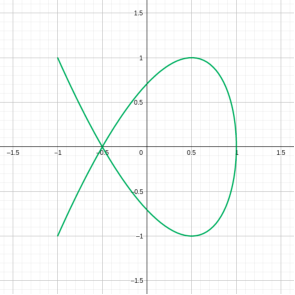
\includegraphics{resources/oplossing57a}
		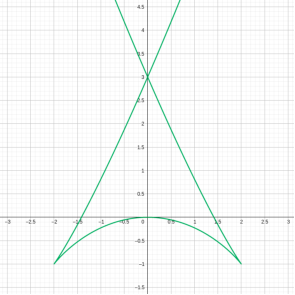
\includegraphics{resources/oplossing57b}
	\end{figure}
\end{problem}

\begin{problem}{58.}
	Met de complexe exponentiële functie en het \textit{binomium van Newton} geldt:
    \begin{equation*}
    \begin{split}
        \sin^{100} x & = {\left( \frac{e^{i x} - e^{- i x}}{2i} \right)}^{100} \\
                     & = \frac{1}{{(2i)}^{100}} \textstyle\sum\limits_{k=0}^{100} \binom{100}{k} \cdot e^{(100 - k) i x} \cdot {(-1)}^k \cdot e^{- k i x} \\
                     & = \frac{1}{2^{100}} \textstyle\sum\limits_{k=0}^{100} \binom{100}{k} \cdot {(-1)}^k \cdot e^{(100 - 2k) i x}.
    \end{split}
    \end{equation*}
    Nemen we de integraal $\int_{0}^{2 \pi}$, dan blijft in het rechterlid, na verwisseling van $\int$ en $\sum$, alleen de middelste term ($k = 50$) over ($\int_{0}^{2 \pi} e^{n i x}\,dx = 0$ voor $n \neq 0$). Dus:
    \begin{equation*}
        \int_{0}^{2 \pi} \sin^{100} x\,dx = \frac{{(-1)}^{50}}{2^{100}} \binom{100}{50} \int_{0}^{2 \pi} e^0\,dx = \frac{100! \cdot \pi}{2^{99} \cdot {50!}^2}.
    \end{equation*}
    Met de \textit{formule van Stirling}, $n! \approx \frac{n^n \sqrt{2 \pi n}}{e^n}$, volgt:
    \begin{equation*}
        \frac{100! \cdot \pi}{2^{99} \cdot {50!}^2} \approx \frac{2 \cdot {100}^{100} \cdot {\left( e^{50} \right)}^2 \cdot \sqrt{200 \pi} \cdot \pi}{2^{100} \cdot {\left( {50}^{50} \right)}^2 \cdot e^{100} \cdot {\left( \sqrt{100 \pi} \right)}^2} = \frac{\sqrt{2 \pi}}{5} \approx \sqrt{\frac{1}{4}} = \frac{1}{2}.
    \end{equation*}
    Dus:
    \begin{equation*}
        \int_{0}^{2 \pi} \sin^{100} x\,dx \approx \frac{1}{2}.
    \end{equation*}
\end{problem}

\clearpage

\begin{problem}{59.}
	We halen logaritmisch afleiden van stal: $(\ln f(x))' = \frac{f'(x)}{f(x)}$, dus $f'(x) = f(x) (\ln f(x))'$, waarbij $'$ differentiatie naar $x$ aangeeft. Aldus $(x^x)' = x^x (\ln x^x)' = x^x (x \ln x)' = x^x (1 \cdot \ln x + x \cdot \nicefrac{1}{x}) = x^x (1 + \ln x)$.\\Neem de integraal $\int_{1}^{10}$. Het linkerlid is $\int_{1}^{10} (x^x)'\,dx = {10}^{10} - 1^1 \approx {10}^{10}$. Het rechterlid is $\int_{1}^{10} x^x (1 + \ln x)\,dx \approx (1 + \ln 10) \int_{1}^{10} x^x\,dx$, omdat $x^x$ zich op $1 \leq x \leq 10$ in de omgeving van $x = 10$ concentreert (zie hieronder de grafiek van de afbeelding $x \mapsto x^x$) en $\ln x$ daar niet sterk varieert ($\frac{\ln 10 - \ln 8}{\ln 10} \approx 0{,}097$). Er volgt $\int_{1}^{10} x^x\,dx \approx \frac{{10}^{10}}{1 + \ln 10} \approx 3 \cdot {10}^9$.
    \begin{figure}
		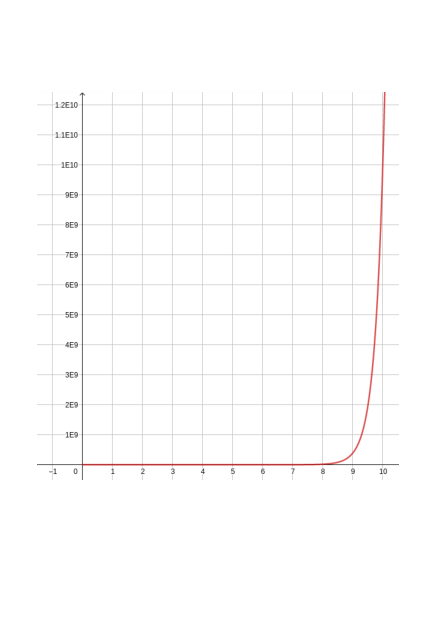
\includegraphics{resources/oplossing59}
	\end{figure}
\end{problem}

\clearpage

\begin{problem}{60.}
	De drie grootcirkels die de driehoek met hoeken $(\alpha,\beta,\gamma)$ bepalen, verdelen het boloppervlak in acht stukken: naast de driehoek zelf zijn dat een identieke, diametraal gelegen driehoek, en nog zes partjes (stukken bolschil bepaald door twee halve grootcirkels tussen twee diametraal gelegen punten op de bol) met één tip afgeknot door één van beide driehoeken (teken dit op een sinaasappel!).

    De oppervlakte van de bol met straal 1 is $4 \pi$. De oppervlakte van een partje van hoek $\phi$ is $(\phi / 2 \pi) \cdot 4 \pi = 2 \phi$ en van een afgeknot partje $2 \phi - S$, waarin $S$ de oppervlakte van de driehoek is. Voor gegeven $(\alpha,\beta,\gamma)$ volgt $S$ uit het gelijkstellen van de acht genoemde stukken aan de bolschil: $S + S + (2 \alpha - S) + (2 \alpha - S) + (2 \beta - S) + (2 \beta - S) + (2 \gamma - S) + (2 \gamma - S) = 4 \pi$, waaruit volgt $S = \alpha + \beta + \gamma - \pi$.
    \begin{figure}
		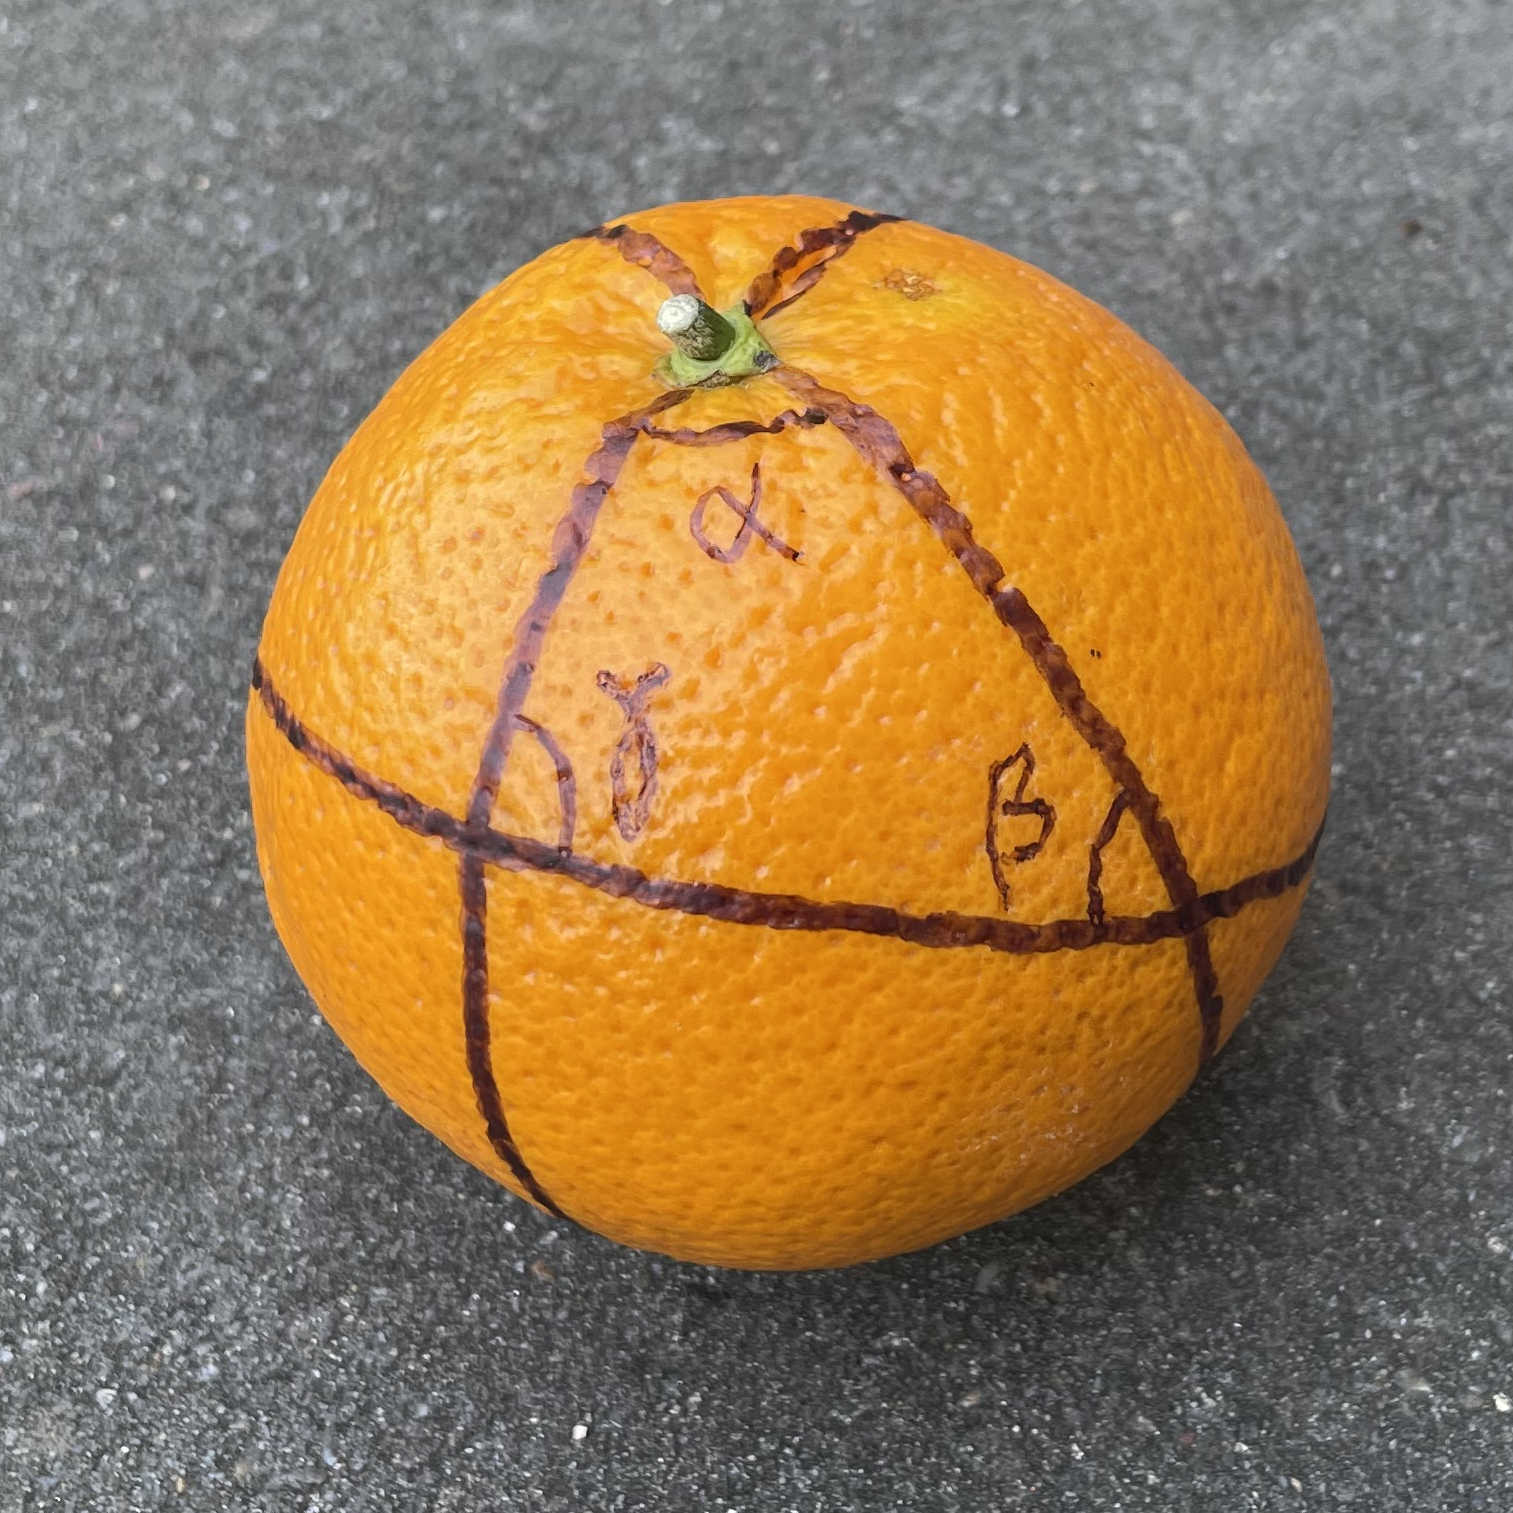
\includegraphics[scale=0.3]{resources/oplossing60}
	\end{figure}
\end{problem}

\begin{problem}{61.}
    Een willekeurig punt $P$ op de rollende kleine cirkel dat op een bepaald moment de grote cirkel raakt, raakt na één omwenteling de grote cirkel opnieuw. De booglengte langs de grote cirkel tussen de twee raakpunten is gelijk aan de omtrek $r = \nicefrac{1}{n}$ van de kleine cirkel. De omtrek van de grote cirkel is $\nicefrac{1}{r} = n$ maal de omtrek van de kleine. De baan van het punt $P$ bestaat dus uit $n$ bogen. In het geval dat $r = \nicefrac{1}{2}$, beweegt $P$ heen en weer over een middellijn van de grote cirkel.
\end{problem}

\clearpage

\begin{problem}{62.}
    De kans dat in een klas van $n$ leerlingen er twee op dezelfde dag jarig zijn is uiteraard 0 voor $n = 1$ en 1 voor $n > 365$ (schrikkeljaren en verjaardagen op 29~februari laten we buiten beschouwing). Het aantal mogelijke verdelingen van $n$ verjaardagen over het jaar is ${365}^n$, en zonder samenvallende verjaardagen $365 \cdot 364 \cdot \dots \cdot (365 - n + 1)$. We nemen aan dat de ene dag niet populairder is als verjaardag dan de andere. De kans op geen samenvallende verjaardagen is dus:
    \begin{equation*}
        p_n = \textstyle\prod\limits_{k=0}^{n-1} \frac{365 - k}{365}.
    \end{equation*}
    Deze kansen zijn achtereenvolgens te berekenen via:
    \begin{equation*}
        p_1 = 1, \text{ } p_n = p_{n-1} \cdot \frac{365 - n + 1}{365} \text{ voor } 2 \leq n \leq 365.
    \end{equation*}
    De kans op samenvallende verjaardagen in een klas van $n$ leerlingen is gelijk aan $1 - p_n$; deze is hieronder uitgezet in een grafiek. Het blijkt dat $p_{23} \approx \nicefrac{1}{2}$, dus $n_0 = 23$. In een klas van 30 leerlingen is de kans op twee jarigen op één dag al $1 - p_{30} \approx 0{,}7$.
    \begin{figure}
        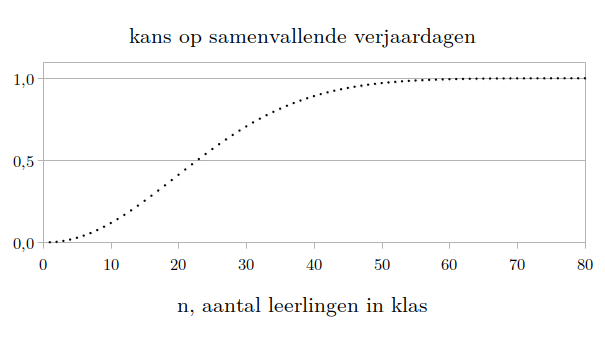
\includegraphics[scale=0.35]{resources/oplossing62}
    \end{figure}
\end{problem}

\clearpage

\begin{problem}{63.}
    De brekingsindex $n(y)$ bereikt een maximum op een zekere hoog\-te $y = y_*$. Een lichtstraal die op een voorwerp weerkaatst in een punt met $y = y_0$ niet te ver van $y_*$ vandaan en onder een uitgaande hoek $\alpha = {\alpha}_0$ met de verticaal, voldoet aan $n(y) \sin \alpha = n(y_0) \sin {\alpha}_0$.

    Omdat $0 < \alpha < \pi$ en dus $0 < \sin \alpha \leq 1$, loopt de lichtstraal binnen de horizontale strook overeenkomend met \mbox{$n(y_0) \sin {\alpha}_0 \leq n(y) \leq n(y_*)$}. Neemt $n(y)$ af, dan neemt $\sin \alpha$ toe, dus neigt $\alpha$ naar $\nicefrac{\pi}{2}$. We conclu\-deren dat de lichtstraal golft in een strook rond $y = y_*$, met langere golven naarmate ${\alpha}_0$ dichter bij $\nicefrac{\pi}{2}$ ligt; voor ${\alpha}_0 = \nicefrac{\pi}{2}$ is de lichtstraal recht.

    (Een waarnemer vormt zich een beeld van het voorwerp op basis van de lichtstralen die in zijn oog vallen, en wel op basis van de richtingen waaronder die golvende lichtstralen invallen. Omdat die golven verschillende golflengten kunnen hebben, kan de verticale on\-derlinge ligging van twee lichtstralen uit twee verschillende punten van het voorwerp bij aankomst in het oog zijn omgekeerd. Het voorwerp lijkt dan ondersteboven te staan.)
\end{problem}

\clearpage

\begin{problem}{64.}
    Dit vraagstuk staat bekend als het \textit{probleem van Fagnano}. We gebruiken een natuurkundig argument, en nemen voor de gegeven driehoek $ABC$ (met hoeken $\alpha,\beta,\gamma$ en zijden met lengten $k,l,m$) een gladde ijzerdraad en voor de gezochte driehoek $KLM$ (met hoeken $\kappa,\lambda,\mu$) een elastiek. Het elastiek neemt vanzelf de minimale lengte aan. Omdat de spankracht in het elastiek in rust overal dezelfde waarde heeft, zijn in elk hoekpunt van $KLM$ de hoeken tussen zijn zijden en de betreffende zijde van $ABC$ gelijk (anders zou het elastiek nog verschuiven totdat de krachten in de punten $K,L,M$ in evenwicht zijn), oftewel de hoekdeellijnen van $\kappa,\lambda,\mu$ staan loodrecht op de zijden van $ABC$.

    Eerst berekenen we de hoeken en zijden van de driehoeken $AKM$, $BKL$, $CLM$. Omdat de hoeken per driehoek optellen tot $\pi$ radialen, geldt het stelsel vergelijkingen $\alpha + \nicefrac{1}{2} (\pi - \kappa) + \nicefrac{1}{2} (\pi - \mu) = \pi$, $\beta + \nicefrac{1}{2} (\pi - \kappa) + \nicefrac{1}{2} (\pi - \lambda) = \pi$, $\gamma + \nicefrac{1}{2} (\pi - \lambda) + \nicefrac{1}{2} (\pi - \mu) = \pi$. Dit heeft als oplossing $\kappa = \alpha + \beta - \gamma$, $\lambda = -\alpha + \beta + \gamma$, $\mu = \alpha - \beta + \gamma$. Omdat ook $\alpha + \beta + \gamma = \pi$, volgt $k = \pi - 2 \gamma$, $\lambda = \pi - 2 \alpha$, $\mu = \pi - 2 \beta$. En hieruit volgt weer dat $AKM$, $BKL$, $CLM$ gelijkvormig zijn met $ABC$, met schaalfactoren resp. $0 < u,v,w < 1$ waarmee de lengten van hun zijden kunnen worden uitgedrukt ten opzichte van $k,l,m$. Voor de lengten van de zijden geldt $k = u m + v l$, $l = v k + w m$, $m = u k + w l$, met oplossing $u = \frac{k^2 + m^2 - l^2}{2 k m}$, $v = \frac{k^2 + l^2 - m^2}{2 k l}$, $w = \frac{l^2 + m^2 - k^2}{2 l m}$.

    Beschouw nu de loodrechte projectie $P$ van het hoekpunt $C$ op de zijde $AB$, op afstand $p$ van $A$ en $q$ van $C$. Toepassen van de stelling van Pythagoras op $ACP$ en op $BCP$, dus $p^2 + q^2 = m^2$ en $(k - p)^2 + q^2 = l^2$, geeft $p = \frac{k^2 + m^2 - l^2}{2 k}$. We zien dat $p = u m$, en dat dus $K = P$. En analoog voor de twee andere hoekpunten.

    Dus de hoekdeellijnen van $\kappa,\lambda,\mu$ staan loodrecht op de zijden van $ABC$ en gaan door zijn hoekpunten, en zijn dus zijn hoogtelijnen. We concluderen dat $KLM$ de voetpuntsdriehoek van het hoogtepunt van $ABC$ is; zijn omtrek bedraagt $u l + v m + w k$.
    \begin{figure}
        \vspace{0.5cm}
        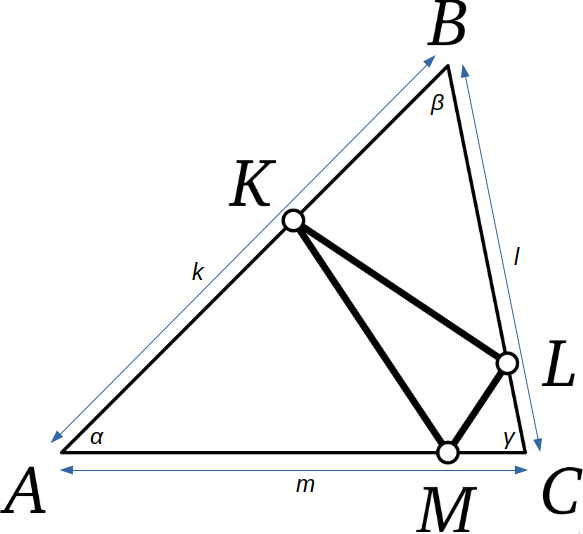
\includegraphics[scale=0.14]{resources/oplossing641}
        \hspace{0.1cm}
        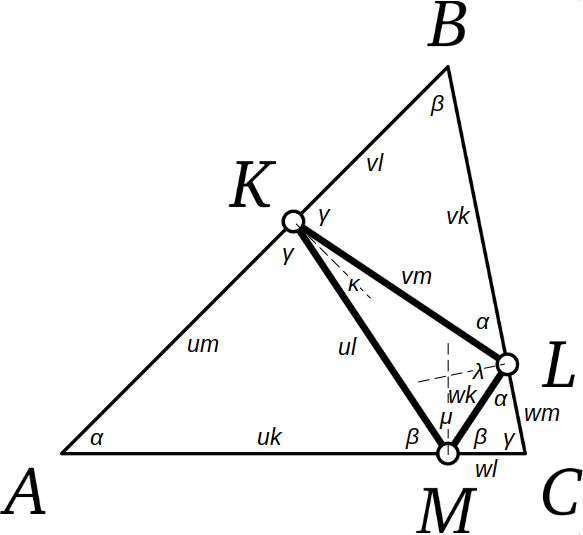
\includegraphics[scale=0.14]{resources/oplossing642}
        \hspace{0.1cm}
        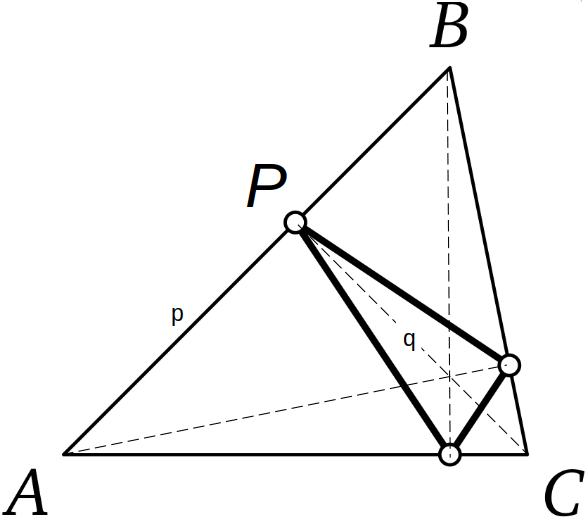
\includegraphics[scale=0.14]{resources/oplossing643}
    \end{figure}
\end{problem}

\clearpage

\begin{problem}{65.}
	In oplossing~26 hebben we gezien dat een strookje van een bol\-schil en de projectie ervan op de cylindermantel die de bol omvat dezelfde opppervlakte hebben. Daaruit volgt dat plakjes van de bol\-schil van gelijke hoogte gelijke oppervlakte hebben. Het gemiddelde van een functie op een bol die per breedtecirkel constant is, is daarom gelijk aan het gemiddelde van die functie over de breedtecirkels.

    Voor de gegeven bol met straal $R$ en middelpunt $(X,Y,Z)$ passen we dit nu toe, waarbij de rechte lijn door de oorsprong $(0,0,0)$ en het punt $(X,Y,Z)$ de as van onze beschouwing vormt. De uitdrukking~$\nicefrac{1}{r}$, waarin $r$ de afstand tot de oorsprong is, wordt als functie over de breedtecirkels gegeven door:
    \begin{equation*}
        r(h) = \sqrt{(\rho + h)^2 + R^2 - h^2} = \sqrt{R^2 + \rho^2 + 2 \rho h},\, -R \leq h \leq R,
    \end{equation*}
    met $\rho = r(X,Y,Z)$.\\
    Merk op dat:
    \begin{equation*}
        r'(h) = \frac{\rho}{r(h)}.
    \end{equation*}
    Hieruit volgt voor het gevraagde gemiddelde op de bol:
    \begin{equation*}
        \overline{\left( \frac{1}{r} \right)} = \frac{1}{2 R} \int_{-R}^{R} \frac{dh}{r(h)} = \frac{1}{2 R \rho} \int_{-R}^{R} r'(h) \,dh = \frac{1}{2 R \rho} (r(R) - r(-R)).
    \end{equation*}
    We onderscheiden het geval dat de oorsprong buiten de bol ligt, $R < \rho$:
    \begin{equation*}
        \dots = \frac{1}{2 R \rho} (\rho + R - (\rho - R)) = \frac{1}{\rho},
    \end{equation*}
    het geval dat de oorsprong binnen de bol ligt, $\rho < R$:
    \begin{equation*}
        \dots = \frac{1}{2 R \rho} (\rho + R - (R - \rho)) = \frac{1}{R},
    \end{equation*}
    en het geval dat de oorsprong op de bol ligt, $\rho = R$:
    \begin{equation*}
        \dots = \lim_{\epsilon \downarrow 0} \frac{1}{2 R} \int_{-R + \epsilon}^{R} \frac{dh}{r(h)} = \dots = \frac{1}{R}.
    \end{equation*}
\end{problem}

\clearpage

\begin{problem}{66.}
	In oplossingen~66 t/m 70 rekenen we met logaritmen. Reken\-regels zijn: $\log_g g = 1$, $\log_g g^b = b$, $\log_g a^b = b \log_g a$, $\log_g (a \cdot b) = \log_g a + \log_g b$, $\log_g \frac{a}{b} = \log_g a - \log_g b$.\\

    Er geldt $10 \log_{10} 2 = \log_{10} 2^{10} = \log_{10} 1024 \approx \log_{10} {10}^3 = 3$, dus $\log_{10} 2 \approx 0{,}3$ is een grove benadering.\\Exact geldt $10 \log_{10} 2 = \log_{10} 2^{10} = \log_{10} 1024 = \log_{10} ({10}^3 \cdot 1{,}024) = \log_{10} {10}^3 + \log_{10} 1{,}024 = 3 + \log_{10} 1{,}024$, dus:
    \begin{equation*}
        \log_{10} 2 = \frac{3}{10} + \frac{1}{10} \log_{10} 1{,}024.
    \end{equation*}
    We zoeken een schatting $\log_{10} 1{,}024 \approx \nicefrac{1}{n}$, voor een natuurlijk getal $n$. Dit betekent ${10}^{\nicefrac{1}{n}} \approx 1{,}024$ oftewel ${1{,}024}^n \approx 10$. We kunnen uitrekenen dat ${1{,}024}^{97} \approx 9{,}979$ en ${1{,}024}^{98} \approx 10{,}219$. Met $\log_{10} 1{,}024 \approx \nicefrac{1}{97} \approx 0{,}01031$ is een betere benadering $\log_{10} 2 \approx 0{,}301$.
\end{problem}

\begin{problem}{67.}
	We gebruiken de benadering $\log_{10} 2 \approx 0{,}301$ uit oplossing~66.

\noindent $\log_{10} 4 = \log_{10} 2^2 = 2 \log_{10} 2 \approx 0{,}602$\\
$\log_{10} 8 = \log_{10} 2^3 = 3 \log_{10} 2 \approx 0{,}903$\\
$\log_{10} 5 = \log_{10} \frac{10}{2} = \log_{10} 10 - \log_{10} 2 \approx 1 - 0{,}301 = 0{,}699$\\
$\log_{10} 50 = \log_{10} (10 \cdot 5) = \log_{10} 10 + \log_{10} 5 \approx 1 + 0{,}699 = 1{,}699$\\
$\log_{10} 32 = \log_{10} 2^5 = 5 \log_{10} 2 \approx 1{,}505$\\
$\log_{10} 128 = \log_{10} 2^7 = 7 \log_{10} 2 \approx 2{,}107$\\
$\log_{10} 125 = \log_{10} 5^3 = 3 \log_{10} 5 \approx 2{,}097$\\
$\log_{10} 64 = \log_{10} 2^6 = 6 \log_{10} 2 \approx 1{,}806$
\end{problem}

\begin{problem}{68.}
	Er geldt dat $2 \log_{10} 7 = \log_{10} 7^2 = \log_{10} 49 \approx \log_{10} 50$, dus $\log_{10} 7 \approx \frac{1}{2} \log_{10} 50$. In oplossing~67 zagen we dat $\log_{10} 50 \approx 1{,}699$. Dus $\log_{10} 7 \approx 0{,}850$.
\end{problem}

\begin{problem}{69.}
	Er geldt $\log_{10} 9 + \log_{10} 7 = \log_{10} (9 \cdot 7) = \log_{10} 63 \approx \log_{10} 64$. We zagen $\log_{10} 64 \approx 1{,}806$ en $\log_{10} 7 \approx 0{,}850$, in respectievelijk oplossin\-gen~67 en 68. Er volgt $\log_{10} 9 \approx \log_{10} 64 - \log_{10} 7 \approx 0{,}956$. We gebruiken ook de benadering $\log_{10} 2 \approx 0{,}301$ uit oplossing~66.

\noindent $\log_{10} 3 = \log_{10} \sqrt{9} = \frac{1}{2} \log_{10} 9 \approx 0{,}478$\\
$\log_{10} 27 = \log_{10} 3^3 = 3 \log_{10} 3 \approx 1{,}434$\\
$\log_{10} 6 = \log_{10} (2 \cdot 3) = \log_{10} 2 + \log_{10} 3 \approx 0{,}779$\\
$\log_{10} 12 = \log_{10} (2^2 \cdot 3) = 2 \log_{10} 2 + \log_{10} 3 \approx 1{,}080$
\end{problem}

\clearpage

\begin{problem}{70.}
	Neem twee natuurlijke getallen $m$ en $n$ die ongeveer even groot zijn: $\frac{m}{n} = 1 + \frac{m - n}{n} \approx 1$ en $0 < \lvert \frac{m - n}{n} \rvert \ll 1$.

    Er geldt $\log_{10} \frac{m}{n} = \log_{10} m - \log_{10} n$.

    Met de gegeven betrekking en de lineaire benadering geldt ook $\log_{10} \frac{m}{n} = \log_{10} (1 + \frac{m - n}{n}) = \frac{1}{\ln 10} \cdot \ln (1 + \frac{m - n}{n}) \approx \frac{1}{\ln 10} \left( \frac{m - n}{n} \right)$.

    Er volgt:
    \begin{equation*}
    	\ln 10 \approx \frac{m - n}{n (\log_{10} m - \log_{10} n)}.
    \end{equation*}

    Verder geldt met de gegeven betrekking en $\ln e = \log_e e = 1$:
    \begin{equation*}
	    \log_{10} e = \frac{\ln e}{\ln 10} = \frac{1}{\ln 10}.
    \end{equation*}

    Voor $m = 1024$, $n = 1000$, en met de benadering $\log_{10} 1{,}024 \approx \nicefrac{1}{97}$ uit oplossing~66, volgt: $\ln 10 \approx 2{,}328$ en $\log_{10} e \approx 0{,}430$.\\

    [Als we een getal $y$ benaderen met een product van steunpunten~$y_i$ met bekende $\log_{10} y_i$, $i = 1,\dotsc,n$, dan is $y = (1 + x) \prod\limits_{i=1}^{n} y_{i}$ voor een zekere kleine $x$, en:
    \begin{equation*}
    \begin{split}
		\log_{10} y & = \log_{10} \left( (1 + x) \textstyle\prod\limits_{i=1}^{n} y_{i} \right) \\
		            & = \textstyle\sum\limits_{i=1}^{n} \log_{10} y_{i} + \log_{10} (1 + x) \\
		            & = \textstyle\sum\limits_{i=1}^{n} \log_{10} y_{i} + \frac{\ln (1 + x)}{\ln 10} \\
		            & \approx \textstyle\sum\limits_{i=1}^{n} \log_{10} y_{i} + \frac{1}{\ln 10} \left( x - \frac{x^2}{2} + \frac{x^3}{3} - \frac{x^4}{4} + \dotsb \right).]
    \end{split}
	\end{equation*}
\end{problem}

\clearpage

\begin{problem}{71.}
    We gebruiken de \textit{Equidistributiestelling van Weyl}: Voor elk ir\-rationaal getal $\alpha$ zijn de decimale delen van de getallen $\alpha,2 \alpha,3 \alpha,\dotsc$ gelijkmatig verdeeld over het interval tussen~0~en~1; het percentage van deze decimale delen op een willekeurig deelinterval is evenredig aan de lengte ervan. Het bewijs is niet eenvoudig en kort. We verwijzen naar de literatuur.\\

    Dat een reëel getal $x \geq 1$ begint met het cijfer $k$, $k = 1,2,\dotsc,9$, betekent:
    \begin{equation*}
        k \cdot {10}^n \leq x < (k + 1) \cdot {10}^n,
    \end{equation*}
    voor een zeker geheel getal $n \geq 0$. Om de machten te kunnen hanteren, nemen we hun logaritmen. Daarvoor gelden dezelfde ongelijkheden, daar de logaritme een strikt monotoon stijgende functie is. Dus:
    \begin{equation*}
        0 \leq \log_{10} k \leq \log_{10} x - n < \log_{10} (k + 1) \leq 1,
    \end{equation*}
    oftewel het decimale deel van het getal $\log_{10} x$ ligt tussen $\log_{10} k$ en $\log_{10} (k + 1)$. De getallen $\log_{10} k$ verdelen het interval van~0~tot~1 in negen deelintervallen:
    \begin{equation*}
        0 = \log_{10} 1 < \log_{10} 2 < \dots < \log_{10} 9 < \log_{10} 10 = 1.
    \end{equation*}

    Laat nu $x$ over de machten van~2 lopen, dus $x = 2^m$, $m \geq 0$ geheel, en $\log_{10} x = \log_{10} 2^m = m \log_{10} 2$. Toepassing van de \textit{Equidistributie\-stelling van Weyl} met $\alpha = \log_{10} 2$ (is irrationaal, want $\log_{10} 2 = \frac{a}{b}$ zou betekenen dat $2^a = {10}^b = 2^b \cdot 5^b$, strijdig met de eenduidigheid van de priemfactorontbinding) leidt tot de conclusie dat de kans $p_k$ dat een macht van~2 met het cijfer $k$ begint, gelijk is aan:
    \begin{equation*}
        p_k = \log_{10} (k + 1) - \log_{10} k = \log_{10} \left( 1 + \frac{1}{k} \right),
    \end{equation*}
    dus $p_1 \approx 0{,}301$, $p_2 \approx 0{,}176$, $p_3 \approx 0{,}125$, $p_4 \approx 0{,}097$, $p_5 \approx 0{,}079$, $p_6 \approx 0{,}067$, $p_7 \approx 0{,}058$, $p_8 \approx 0{,}051$, $p_9 \approx 0{,}046$, en vanzelfsprekend is $\Sigma_{k=1}^{9} p_k = 1$.
\end{problem}

\begin{problem}{72.}
	Analoog aan oplossing~71 (bedenk dat ook $\log_{10} 3$ irrationaal is, immers $\log_{10} 3 = \frac{a}{b}$ zou betekenen dat $3^a = 2^b \cdot 5^b$, wat onmogelijk is).
\end{problem}

\clearpage

\begin{problem}{73.}
    Wat hier staat is dat hoe vaak de afbeelding $g$ ook wordt toe\-gepast, er altijd een punt $x$ in $U$ is dat weer in $U$ terugkeert.

    Beschouw de oneindige rij beelden $g^{j N}(U)$, $j \geq 0$, van $U$. Omdat de omgeving $U$ een oppervlakte groter dan 0 heeft en $g$ oppervlakte\-bewarend is, overlappen sommige $g^{j N}(U)$. Zonder overlap zou hun gezamenlijke oppervlakte immers oneindig zijn, terwijl $M$ begrensd is. Er zijn dus zekere $k$ en $l$, $0 \leq k < l$, waarvoor $g^{k N}(U)$ en $g^{l N}(U)$ overlappen. Neem een punt $z$ in hun doorsnede. Hiervoor bestaan punten $x$ en $y$ in $U$ zodat $g^{l N}(x) = g^{k N}(y) = z$. Omdat $g$ injectief is, kunnen we $k N$ keer teruggaan. Dan volgt $g^{(l - k) N}(x) = y$. Dus er is een $x$ in $U$ waarvoor $g^T(x)$, $T = (l - k) N \geq N$, weer in $U$ ligt.
\end{problem}

\begin{problem}{74.}
    Eerst bewijzen we dat de afbeelding $g(\alpha,\beta) = (\alpha + 1,\beta + \sqrt{2}) \pmod {2 \pi}$ geen periodieke punten heeft. Het verschil tussen twee ite\-raties $g^T(\alpha,\beta)$ en $g^{T + t}(\alpha,\beta)$, $T \geq 0$ en $t \geq 1$, van een punt $(\alpha,\beta)$ is gelijk aan $(t,t \sqrt{2}) \pmod {2 \pi}$. Dit is nooit gelijk aan $(0,0)$, $(0,.)$ of $(.,0)$, want gehele veelvouden van 1, $\sqrt{2}$ en $\pi$ zijn opgeteld nooit gelijk aan 0 (1 is geheel, $\sqrt{2}$ irrationaal en algebraïsch, en $\pi$ transcendent). Dus iteraties vallen niet samen, en liggen ook niet recht naast of onder elkaar.

    De afbeelding $g$ is eenvoudigweg een verschuiving, dus het volstaat de dichtheid te bewijzen van de rij iteraties van één bepaald beginpunt, zeg $(0,0)$. Omdat de punten van de rij $\{g^T(0,0)\}$, $T \geq 0$, allen verschil\-lend zijn en de torus een eindige oppervlakte heeft, zijn er $g^M(0,0)$ en $g^{M + N}(0,0)$, met zekere $M \geq 0$ en $N \geq 1$, die willekeurig dicht bij elkaar liggen. Daar $g$ een verschuiving is, liggen de punten van de deelrij $\{g^{N T}(0,0)\}$ op onderling gelijke, willekeurig kleine afstanden op een lijn die zich om de torus windt met helling $\lambda = \frac{\Delta \alpha}{\Delta \beta} = \frac{N - 2 K \pi}{N \sqrt{2} - 2 L \pi}$, voor zekere $K,L \geq 0$. Merk op dat $0 < \lvert \lambda \rvert < \infty$, en dat $\lambda$ irrationaal is, want $p (N \sqrt{2} - 2 L \pi) = q (N - 2 K \pi)$ heeft geen oplossing voor gehele $p$ en $q$.

    Deze lijn snijdt $(\alpha,0)$, $0 \leq \alpha < 2 \pi$, in $(2 \pi \lambda j,0) \pmod {2 \pi}$, $j \geq 0$. Analoog aan het bovenstaande kan worden beredeneerd dat de ite\-raties $h^{j}_{\lambda}(0) = 2 \pi \lambda j \pmod {2 \pi}$, $j \geq 0$, van de verschuiving $h_{\lambda}(\alpha) = \alpha + 2 \pi \lambda \pmod {2 \pi}$ allen verschillend zijn (want gehele veelvouden van~1 en het irrationale getal $\lambda$ zijn opgeteld nooit gelijk aan 0) en er een deelrij is met onderling gelijke, willekeurig kleine afstanden; dit is de \textit{Stelling van Jacobi}. De lijn windt zich dus dicht om de torus.

    Samenvattend zien we dat de deelrij $\{g^{N T}(0,0)\}$ en daarmee de rij $\{g^T(0,0)\}$ dicht ligt in de torus.
\end{problem}

\clearpage

\begin{problem}{75.}
    De afbeelding $g(\alpha,\beta) = (2 \alpha + \beta,\alpha + \beta) \pmod {2 \pi}$ staat bekend als \textit{Arnold's CAT map} (Continu Automorfisme van de Torus) of als \textit{Arnold's cat map} (Arnold gebruikte ter illustratie een tekening van een kattengezicht) of ook wel als \textit{Thom map}.

    Beschouw de punten op de torus geënt op de gelijknamige breuken tussen 0 en 1 met een bepaalde noemer $n$: $x = (\alpha,\beta) = \left( 2 \pi \cdot \frac{a}{n},2 \pi \cdot \frac{b}{n} \right)$, $0 \leq a,b < n$. Omdat $g$ een lineaire afbeelding is met geheeltallige coëfficienten, zijn alle iteraties $g^j(x)$, $j \geq 0$, van deze vorm. Omdat er precies $n^2$ van deze punten zijn, bestaan er voor elke $x$ onder de eerste $n^2 + 1$ iteraties twee samenvallende: $g^{N(x)}(x) = g^{M(x)}(x)$, \mbox{$0 \leq M(x) < N(x) \leq n^2$}. De afbeelding $g$ heeft een inverse, te weten $g^{-1}(\alpha,\beta) = (\alpha - \beta,-\alpha + 2 \beta)$. Teruggaan via $g^{-M(x)}$ geeft $g^{T(x)}(x) = x$, $T(x) = N(x) - M(x)$, dus $x$ is een periodiek punt van de afbeelding~$g$ met periode $0 < T(x) \leq n^2$.

    We zien dat alle $x$ periodieke punten van $g$ zijn. Loopt $n$ over de natuurlijke getallen, dan bestrijken de breuken met noemer $n$ in de definitie van $x$ alle rationale getallen tussen 0 en 1. Zoals bekend liggen de rationale getallen dicht in de reële getallen. Alle aangeduide periodieke punten samen liggen bijgevolg dicht in de torus.
\end{problem}

\begin{problem}{76.}
	???
\end{problem}

\begin{problem}{77.}
	???
\end{problem}

\clearpage

\null\vfill
\noindent
Oplossingen in het Nederlands:\\
\null\quad Rik Biel\\
\\
Versie:\\
\null\quad \today\\
\\
\\
\\
Oorspronkelijk Russisch opgavenboek van V.\,I.~Arnold:\\
\null\quad \textrussian{В. И. Арнольд: Задачи для детей от 5 до 15 лет}\\
\null\quad Moskou, MCCME, 2004\\
\null\quad ISBN 5-94057-183-2

\end{document}
